\chapter{Search for supersymmetry using boosted Higgs bosons and missing transverse momentum in proton-proton collisions at 13 TeV}
\label{chap:analysis}

\section{Motivation \& Introduction}

As the masses of potentially new particles are pushed to larger and larger scales \cite{CMS-SUS-16-033} \cite{CMS-SUS-15-002}. This results in any Standard Model (SM) particles radiated during their decay having correspondingly larger momentum (high boost). As a particle becomes more boosted its decay products are emitted at smaller angles, eventually collimating sufficiently to be reconstructed as a single jet. If new physics exists with masses achievable by the LHC, one could suspect that there exists non-zero coupling with the electroweak H, Z, or W bosons. Observation of events containing high-$p_{T}$ ($>$300 GeV) electroweak bosons are thus of considerable interest for potential SUSY signals. 

The Minimal Supersymmetric Standard Model contains a $\mathbb{Z}_{2}$ symmetry in which all SM particles have charge -1 and all supersymmetric particles have charge +1, this is called R-parity\cite{susyprimer}. One direct consequence of R-parity is that the decay of a massive supersymmetric particle must include at least one supersymmetric particle in the final state. Necessarily this is the lightest such particle in the theory, denoted the lightest supersymmetric particle (LSP). If the LSP is electrically neutral it may escape detection, creating an imbalance in the net momentum of the event (as would a neutrino). Events with a large momentum imbalance are also interesting as potential regions for SUSY signals.

With this as motivation, we designed an analysis searching for hints of new physics beyond the Standard Model in events with boosted H or Z bosons and a large transverse momentum imbalance of the event. We reconstruct the H and Z bosons in the $\mathrm{b}\bar{\mathrm{b}}$ channel, with 57\% and 15\% branching fractions respectively. Although our analysis is sensitive to any new physics with this final state, we have adopted two benchmark models (known as SMS models\cite{CMS-SUS-11-016}), seen in Figure \ref{fig:sms}, to give motivation to the analysis. In this scenario, the proton-proton interaction produces a pair of gluinos $\tilde{g}$ which decay to a neutralino $\tilde{\chi}_{2}^{0}$ by the emission of Standard Model quarks. A small mass splitting between the gluino and neutralino $\tilde{\chi}_{2}^{0}$ will result in low-$p_{T}$ quarks and a high-$p_{T}$ neutralino $\tilde{\chi}_{2}^{0}$. This neutralino $\tilde{\chi}_{2}^{0}$ further decays into another neutralino $\tilde{\chi}_{1}^{0}$ with the emission of a H or Z boson. The neutralino $\tilde{\chi}_{1}^{0}$ escapes detection.

Past searches targeting similar final states (but different production scenario) have been performed in which the H bosons are produced with low-$p_{T}$, in this case the H bosons are reconstructed as a pair of b-tagged AK4 jets \cite{CMS-SUS-16-044}.
 
\begin{figure}[htbp] 
\begin{subfigure}[b]{0.5\textwidth}
\centering
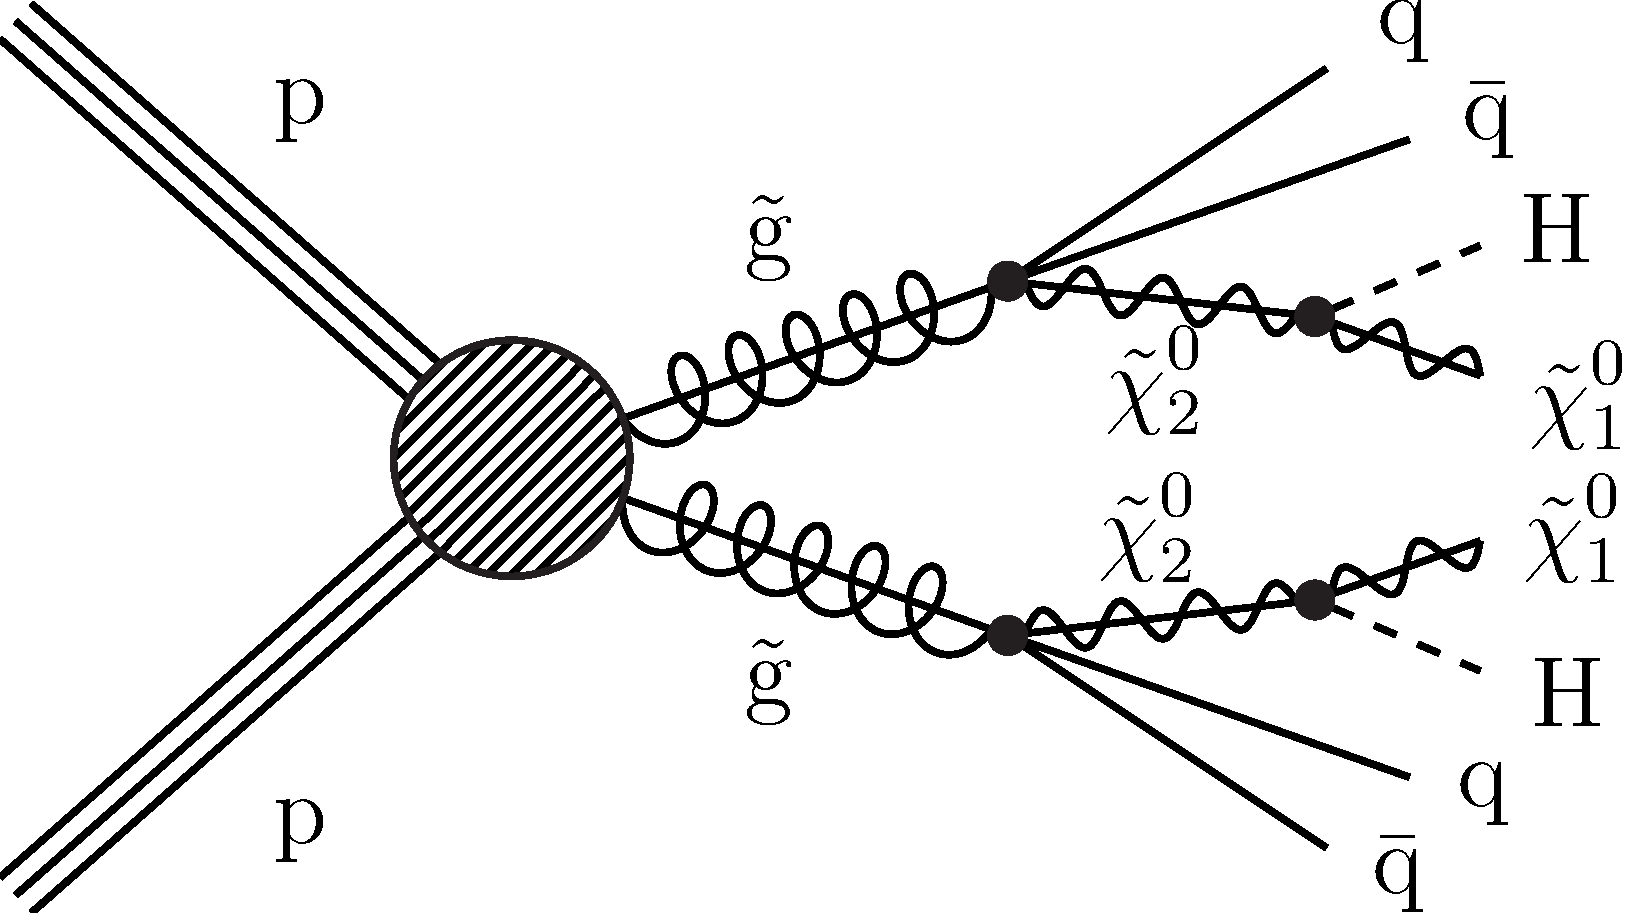
\includegraphics[width=\textwidth]{figs/SUS17006/CMS-SUS-17-006_Figure_001.pdf}
\caption{The T5HH model.}
\label{fig:t5hh}
\end{subfigure}
\begin{subfigure}[b]{0.5\textwidth}
\centering
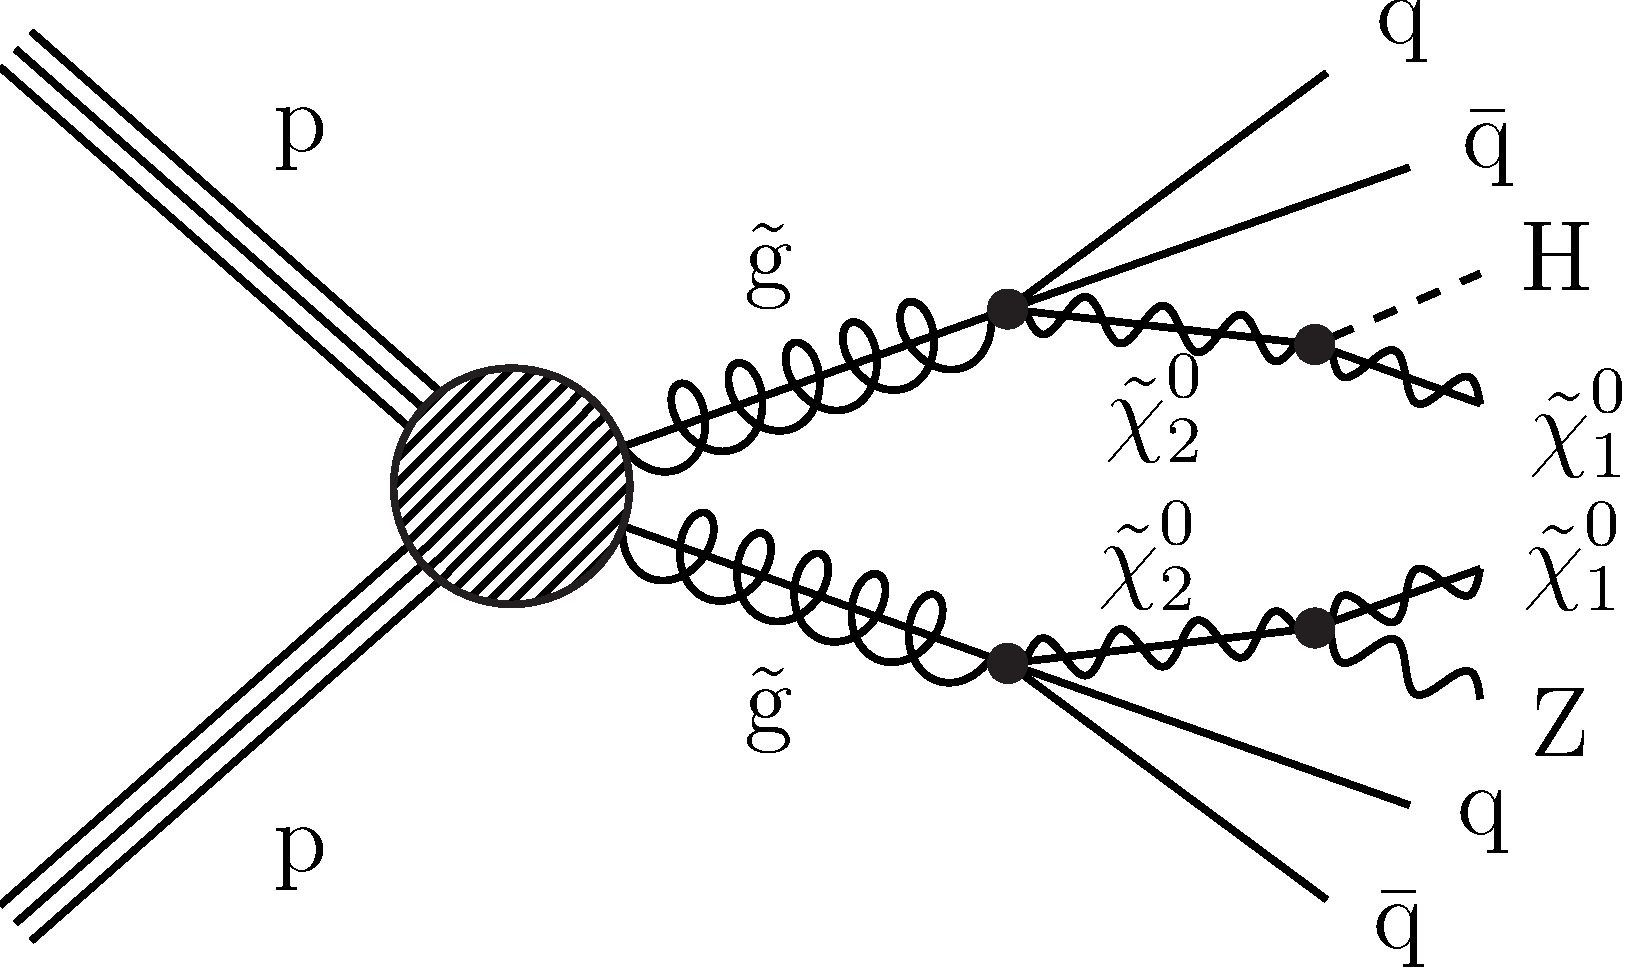
\includegraphics[width=\textwidth]{figs/SUS17006/CMS-SUS-17-006_Figure-aux_001.pdf}
\caption{The T5ZH model.}
\end{subfigure}
\caption{Diagrams of the benchmark models used for motivation of the targeted signal.}
\label{fig:sms}
\end{figure}

\section{Object Definition \& Event Selection}

We establish a baseline selection choosing events with all-hadronic final states and missing transverse momentum, as motivated by Figure \ref{fig:sms} . Our jets are reconstructed using the ``anti-kt`` clustering algorithm with cone sizes of $\Delta R$ = 0.4, 0.8 \cite{1126-6708-2008-04-063}, denoted as AK4 and AK8 jets respectively. AK4 jets subtend less solid angle and are used to capture the hadronisation of single quarks and gluons. AK8 jets subtend a larger solid angle and are used for reconstruction of boosted objects (e.g. $t$, H, Z, W).

The baseline selection is as follows:

\begin{itemize}
\item $\geq2$ AK8 jets; $p_{T} > 300\,\mathrm{GeV}$ and $50 < \mathrm{mass} < 250\,\mathrm{GeV}$
\item $\mathrm{MET} > 300\,\mathrm{GeV}$; $\mathrm{MET}\equiv |-\sum_{\mathrm{PFcandidates}}\vec{p_{T, i}}|$
\item electron veto; $p_{T}>10\,\mathrm{GeV}$, isolated
\item muon veto; $p_{T}>10\,\mathrm{GeV}$, isolated
\item isolated track veto
\item $\Delta\phi_{1, 2, 3, 4} > 0.5, 0.5, 0.3, 0.3$; $\Delta\phi_{i}\equiv \Delta\phi(\vec{\mathrm{MET}}, \mathrm{AK4\,jet}_{i})$\newline
The $\Delta\phi$ cut is designed to mitigate QCD events in which a jet is under-measured leading to an artificial imbalance in the event momentum. This cut requires that the difference in $\phi$ between the MET vector and each of the four leading AK4 jets is sufficiently large to remove events in which a jet has been under-measured giving rise to fake MET pointing in the same direction. If less than four AK4 jets are available the additional cuts are removed.
\end{itemize}

A dedicated heavy tagging algorithm is used to identify AK8 jets arising from the decay of two b quarks. The distribution of the output discriminator for the lead and subleading jets are seen in the left and right panels of Figure \ref{fig:ak8bb}, respectively; signal-like events peak towards larger values. To \bbbar tag the AK8 jets we choose the loose working-point ($>0.3$)corresponding to a signal efficiency of approximately $80\%$ per AK8 jet. The stacked histogram and solid lines shows the distribution after baseline selection for simulation and two representative signal points, respectively.

Further H/Z tagging of an AK8 jet is accomplished by restricting the jet mass window to [85, 135 GeV] to be consistent with that of the H boson. The distributions of the jet mass are seen in Figure \ref{fig:ak8mass}. The signal shown in the solid line is the T5HH model (i.e. Figure \ref{fig:t5hh}). The same identification criteria are applied to tag an AK8 jet as either an H or Z boson, there is no distinction made.

\begin{figure}[htbp]
\begin{subfigure}[b]{0.5\textwidth}
\centering
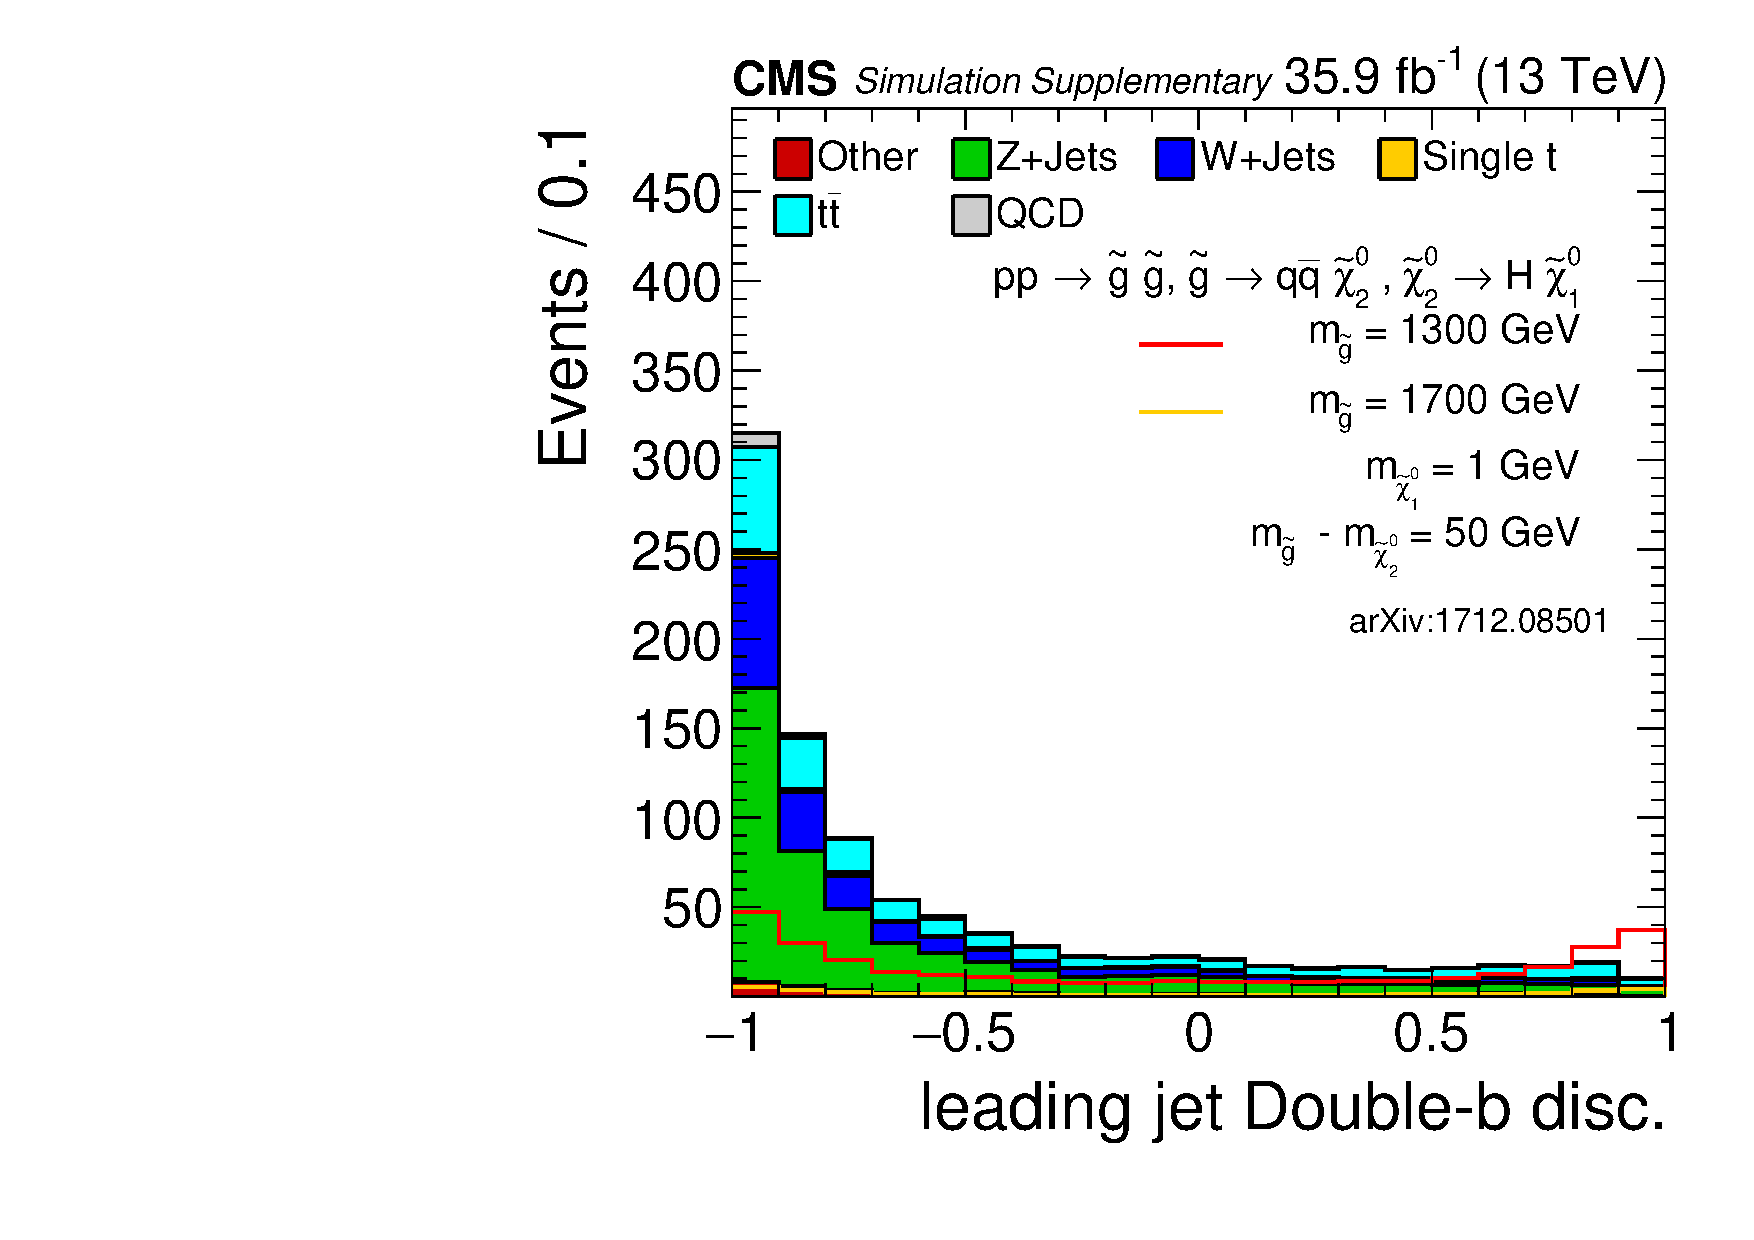
\includegraphics[width=\textwidth]{figs/SUS17006/J1BB_LooseJetMass.pdf}
\end{subfigure}
\begin{subfigure}[b]{0.5\textwidth}
\centering
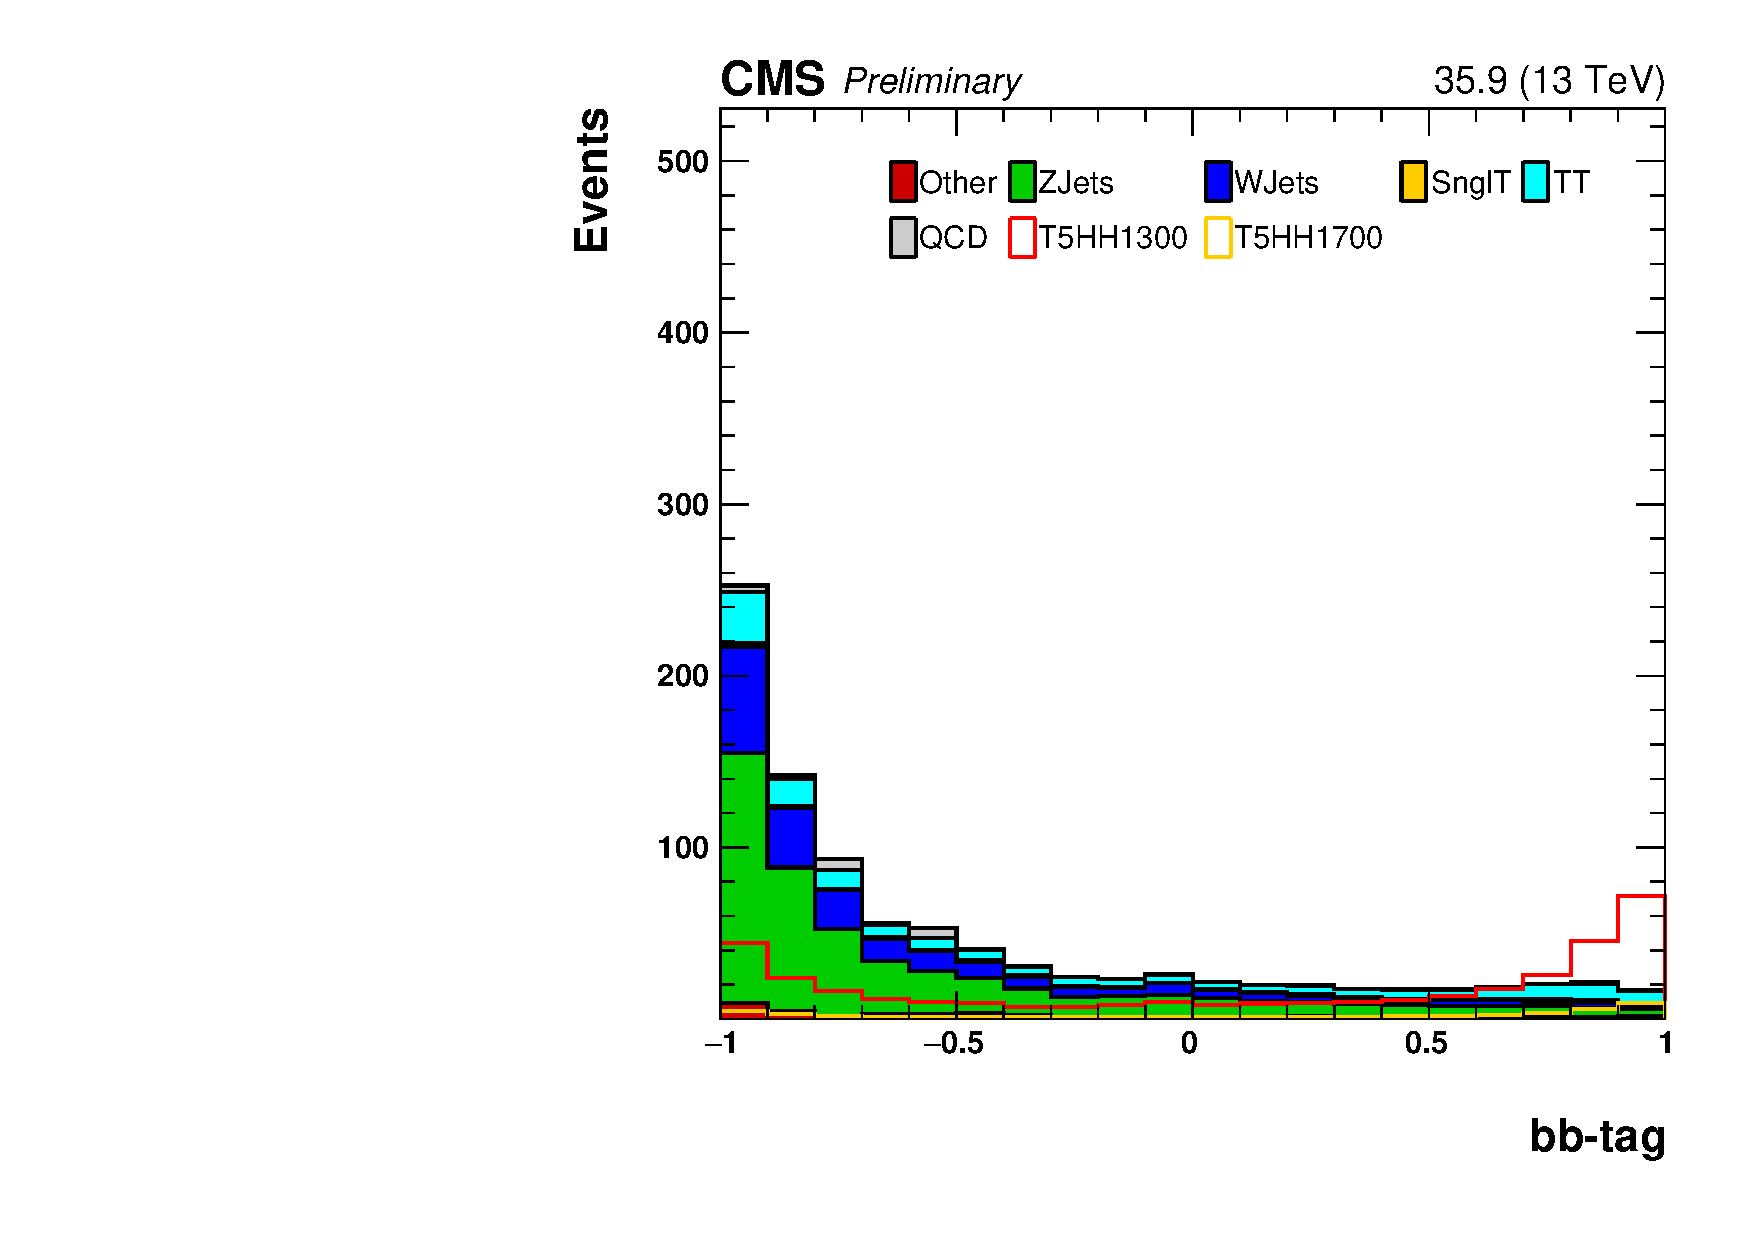
\includegraphics[width=\textwidth]{figs/SUS17006/J2pt_BBtag_baseline.pdf} 
\end{subfigure}
\caption{\bbbar tagging neural network discriminator.}
\label{fig:ak8bb}
\end{figure}

\begin{figure}[htbp]
\begin{subfigure}[b]{0.5\textwidth}
\centering
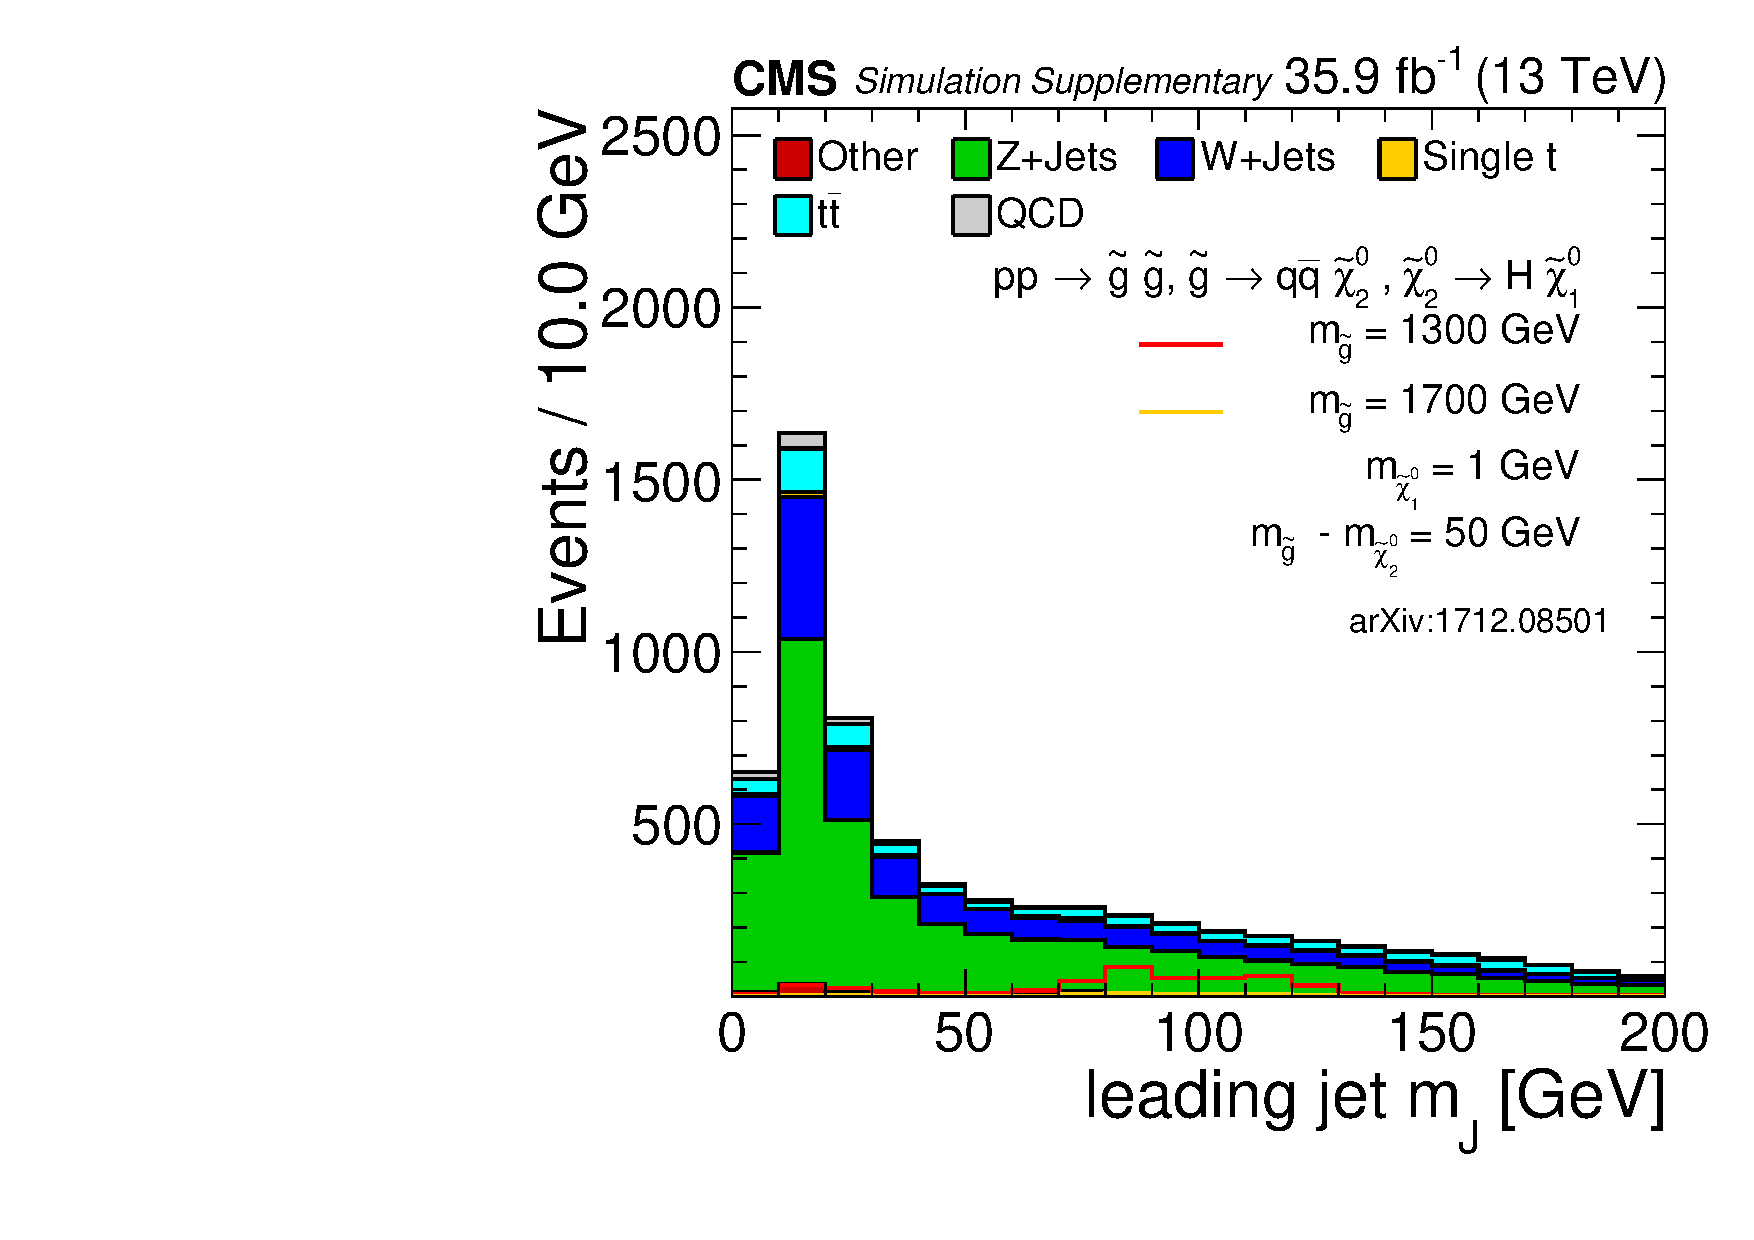
\includegraphics[width=\textwidth]{figs/SUS17006/J1Mwide_JetPt.pdf}
\end{subfigure}
\begin{subfigure}[b]{0.5\textwidth}
\centering
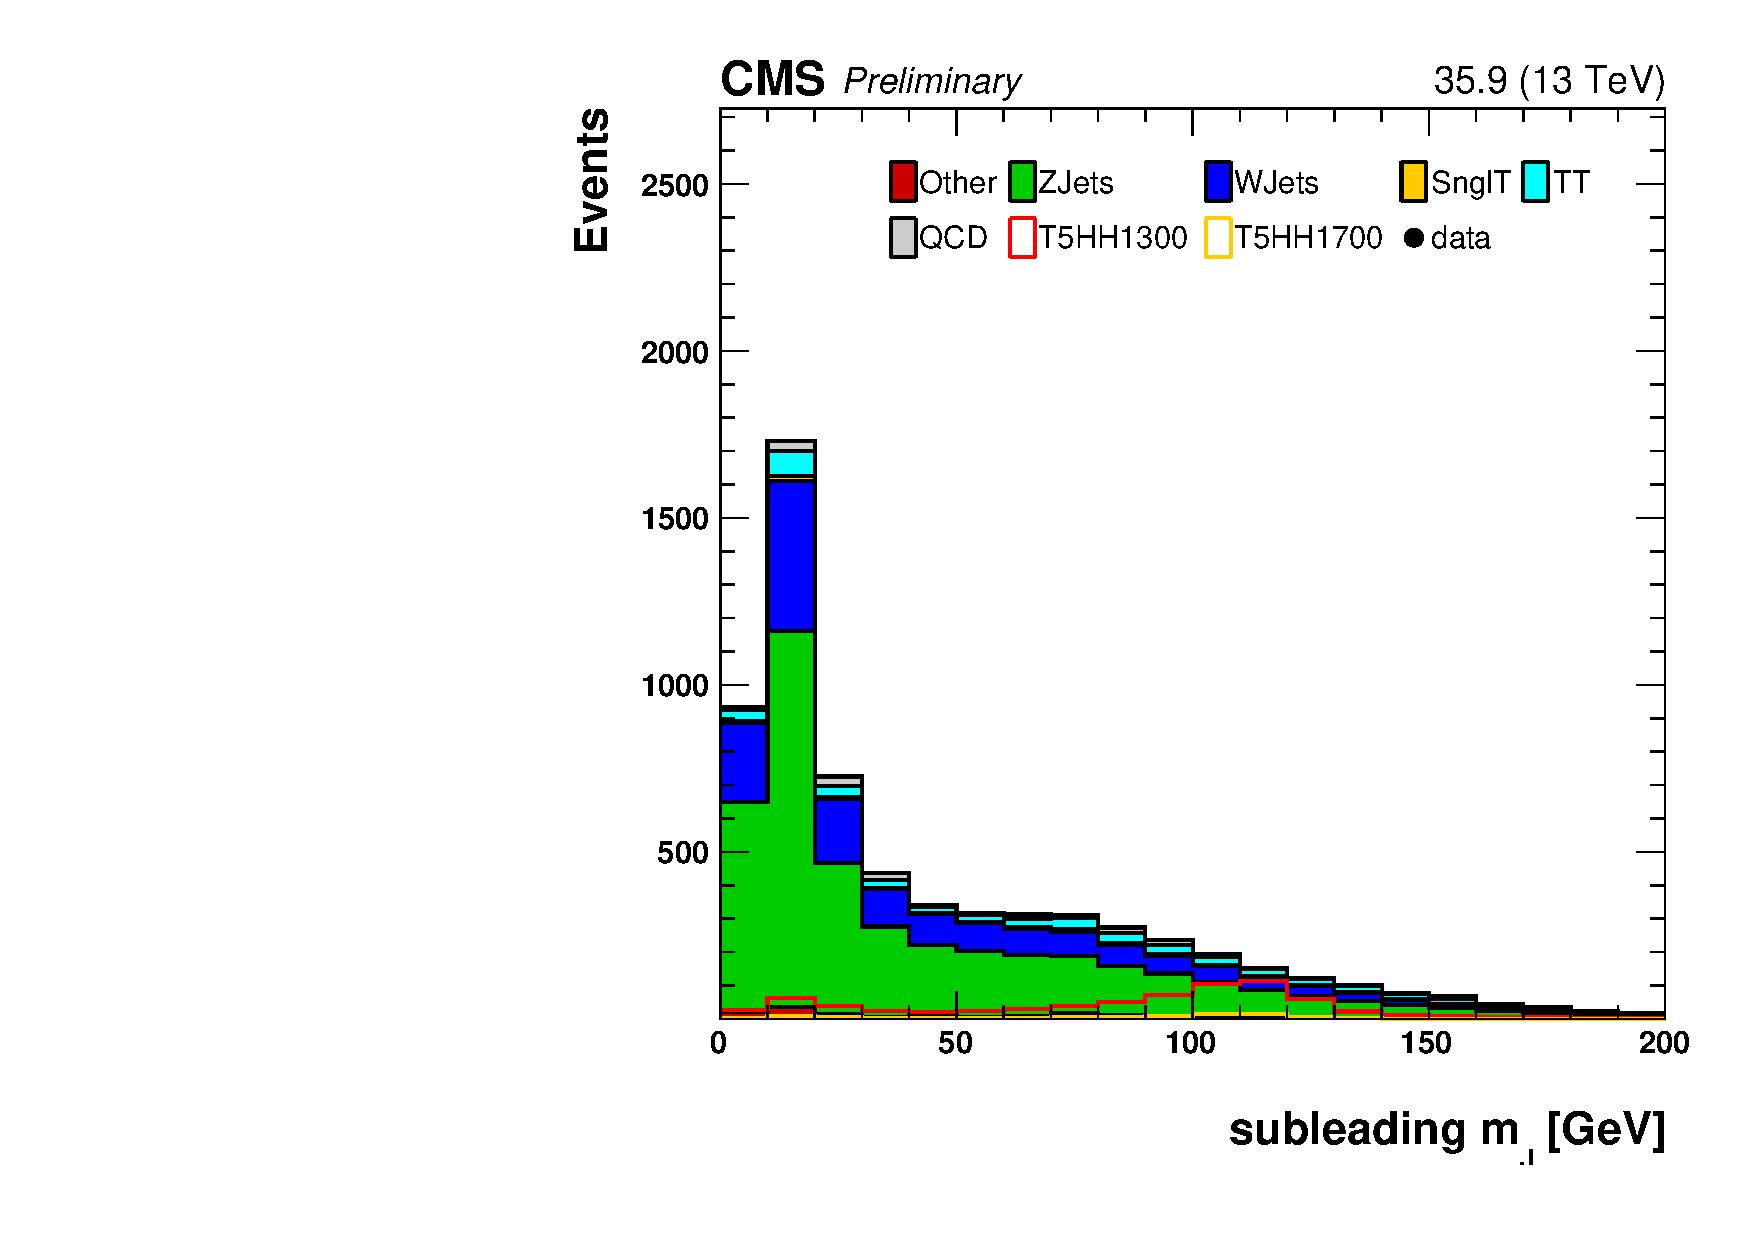
\includegraphics[width=\textwidth]{figs/SUS17006/J2Mwide_JetPt.pdf} 
\end{subfigure}
\caption{The AK8 jet mass.}
\label{fig:ak8mass}
\end{figure}

\section{Dataset and Trigger}

We use a total of 35.9 $fb^{1}$ of data collected by the CMS experiment in 2016. Events are selected in data using a trigger which requires greater than 100 GeV of MET calculated at high-level trigger (HLT); additionally the logical OR of two other triggers with thresholds of 110 and 120 GeV are applied. The trigger efficiency is derived in data using a single-electron reference trigger requiring a tight-ID electron of $p_{T}>27$ GeV. We further select events with at least three AK4 jets and exactly one reconstructed electron of $p_{T}>25$ GeV. The signal region trigger is found to be greater than 98\% for events with MET$>$250 GeV and HT$>$300 GeV \cite{CMS-SUS-16-033}.

\input event-samples.tex

\section{Event Binning \& Background Estimation}

The background estimation procedure makes use of what is known as an ``ABCD'' prediction in which the analysis phase space is divided into signal and sideband regions; scaling relations are applied to sideband yields to make predictions for the SM background (inclusive in all processes) in the signal regions. The events are categorized according to whether the AK8 jets are a) in the signal or sideband mass region and b) have or have not been $\mathrm{b}\bar{\mathrm{b}}$ tagged.  A diagram of this partitioning is seen in Figure \ref{fig:abcd}. An additional dimension is added by binning in MET: [300, 500 GeV], [500, 700 GeV], 700+ GeV. This gives a total of 2x3=6 signal and 4x3=12 sideband bins. The two signal regions $\mathrm{A}_{1}$ and $\mathrm{A}_{2}$ contain events with one (and only one) or two jets being consistent with H/Z boson decay, respectively.

\begin{figure}[htbp]
\centering
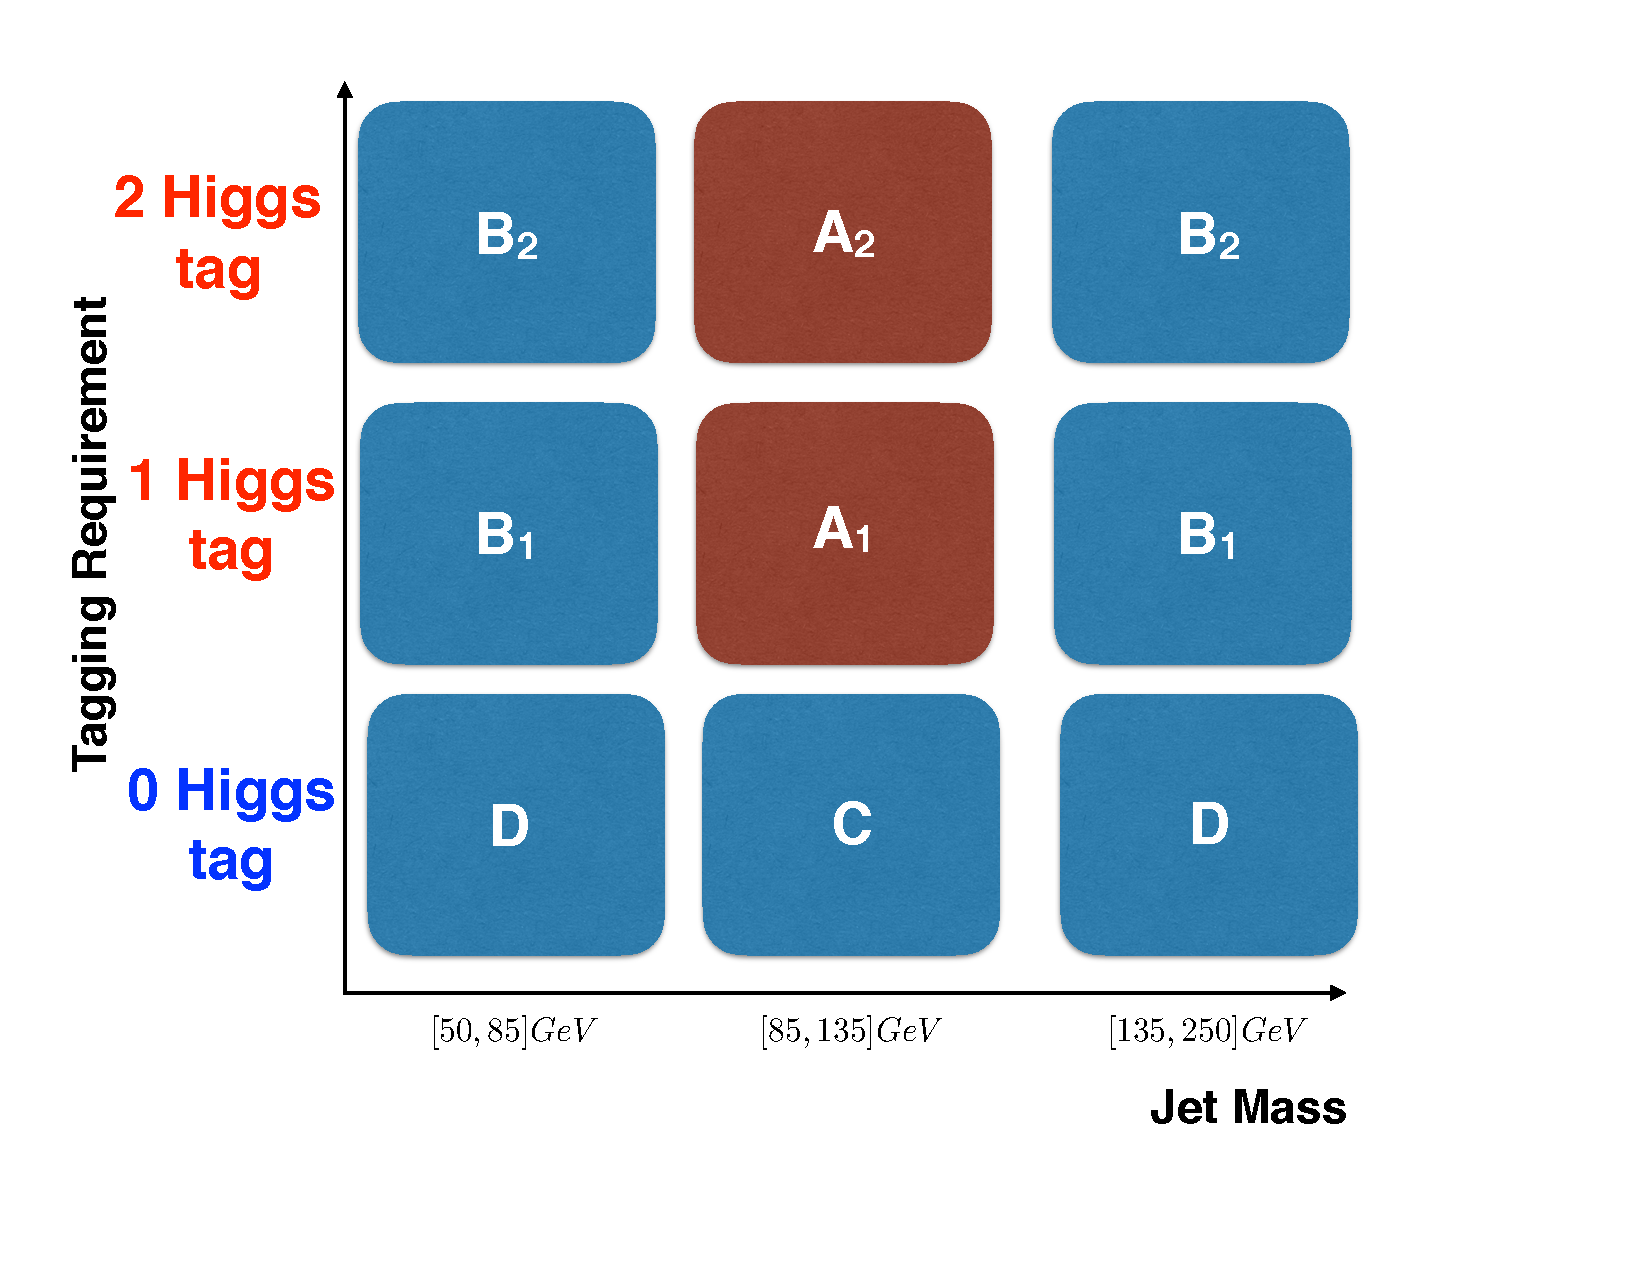
\includegraphics[width=0.6\textwidth]{figs/SUS17006/CMS-SUS-17-006_Figure-aux_002.pdf}
\caption{A diagram of the partitioned phase space. An additional binning in MET brings the number of analysis bins to 6x3=18.}
\label{fig:abcd}
\end{figure}

Assuming that there is no correlation between the jet mass and the \bbbar tagging, the ratio of events $\mathrm{A}_{1, 2} / \mathrm{B}_{1, 2}$ should be the same as $\mathrm{C} / \mathrm{D}$. Rearranging this gives a prediction for the events in the signal regions, $\left(\mathrm{A}_{1, 2}\right)_{\mathrm{prediction}} = \left(\mathrm{B}_{1, 2} * \mathrm{C} / \mathrm{D}\right)_{\mathrm{observed}}$.

The expected MET distribution from simulation is seen in the stacked histograms of Figure \ref{fig:mcclosure}. The prediction using the ABCD method is seen in the red hash. The expected level of closure in simulation can be determined by dividing the prediction in the signal region with the true content. This ratio, denoted $\kappa$, is seen in the bottom panel of Figure \ref{fig:mcclosure}. As will be discussed in Section \ref{sec:kappa}, $\kappa$ is used as a correction in the background estimation procedure.

\begin{figure}[htbp]
\begin{subfigure}[b]{0.5\textwidth}
\centering
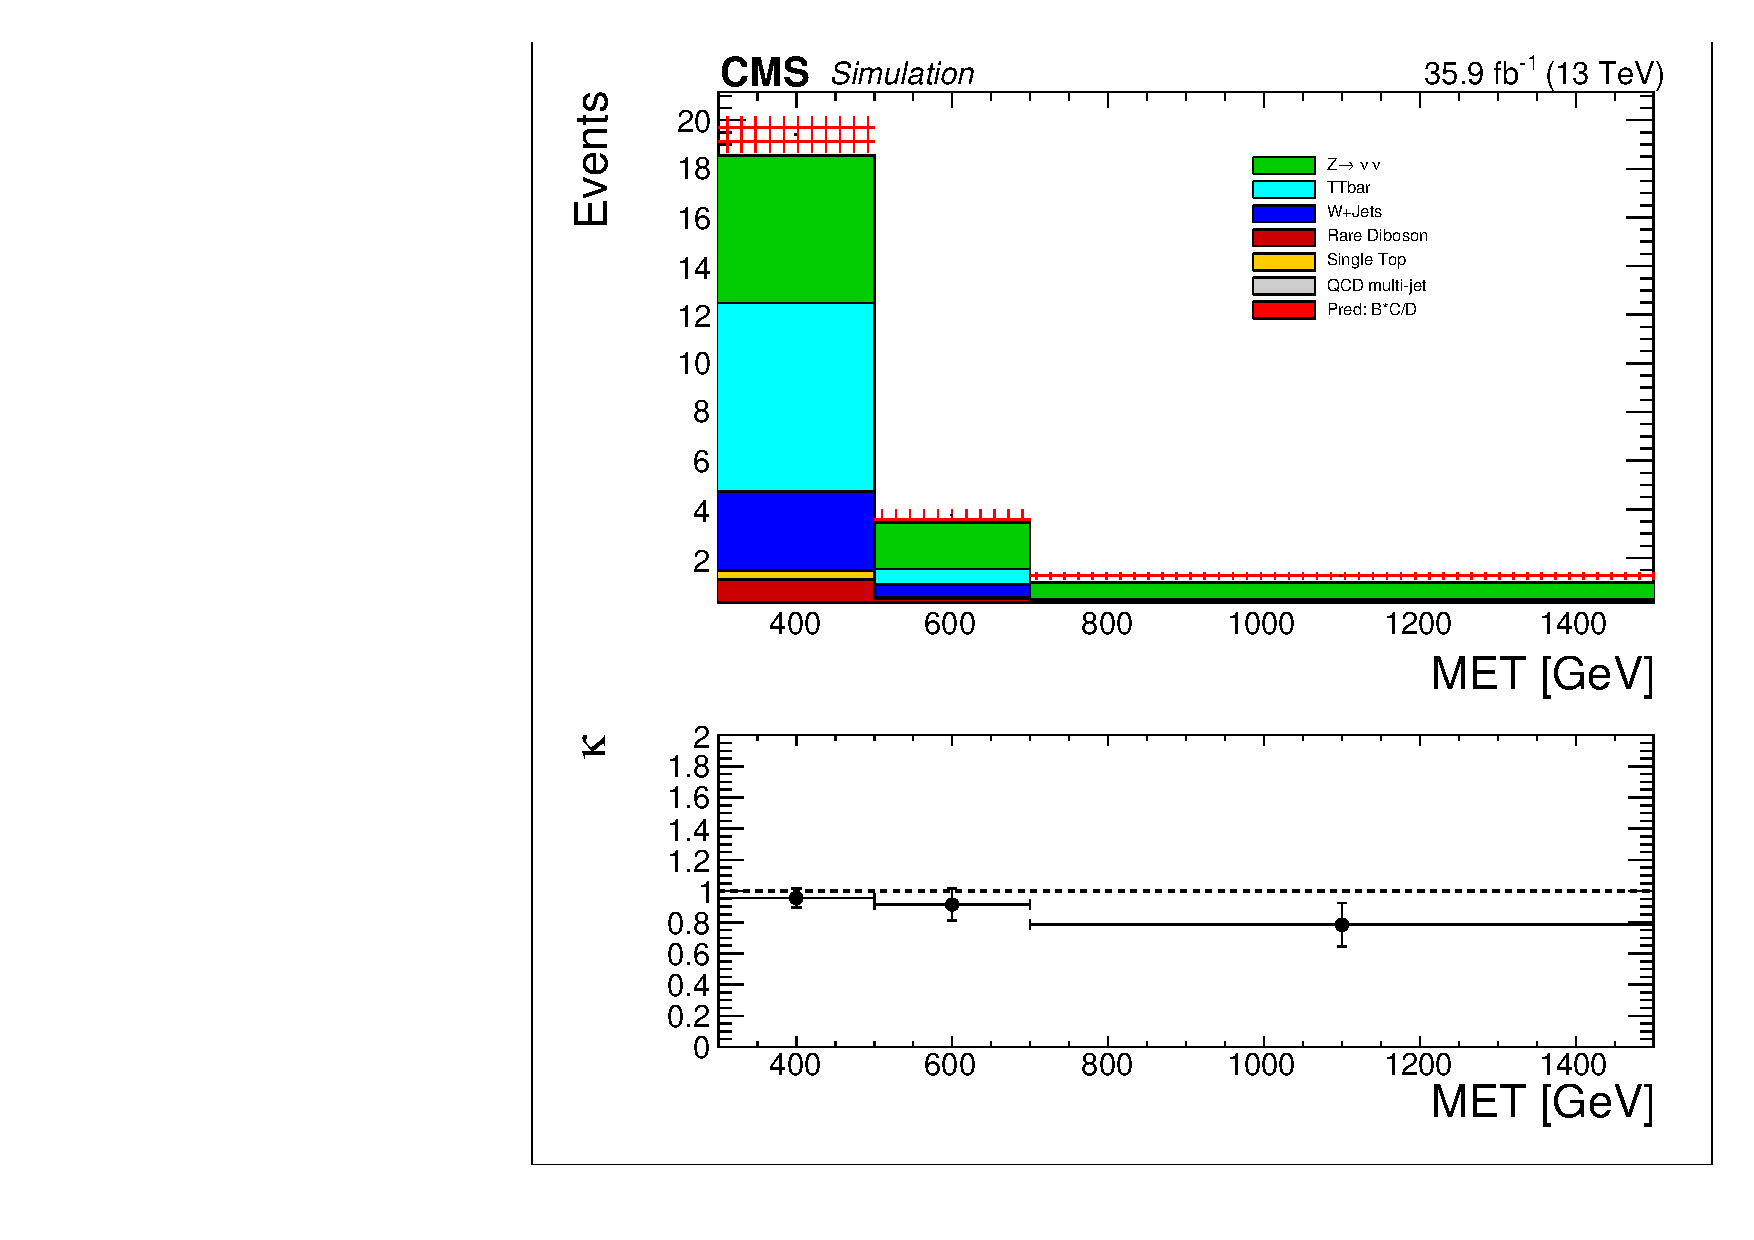
\includegraphics[trim={5px 5px 5px 5px},clip,width=\textwidth]{figs/SUS17006/MCclosure_singleHiggsRegionTotal.pdf}
\caption{The single Higgs tag region (A$_{1}$).}
\end{subfigure}
\begin{subfigure}[b]{0.5\textwidth}
\centering
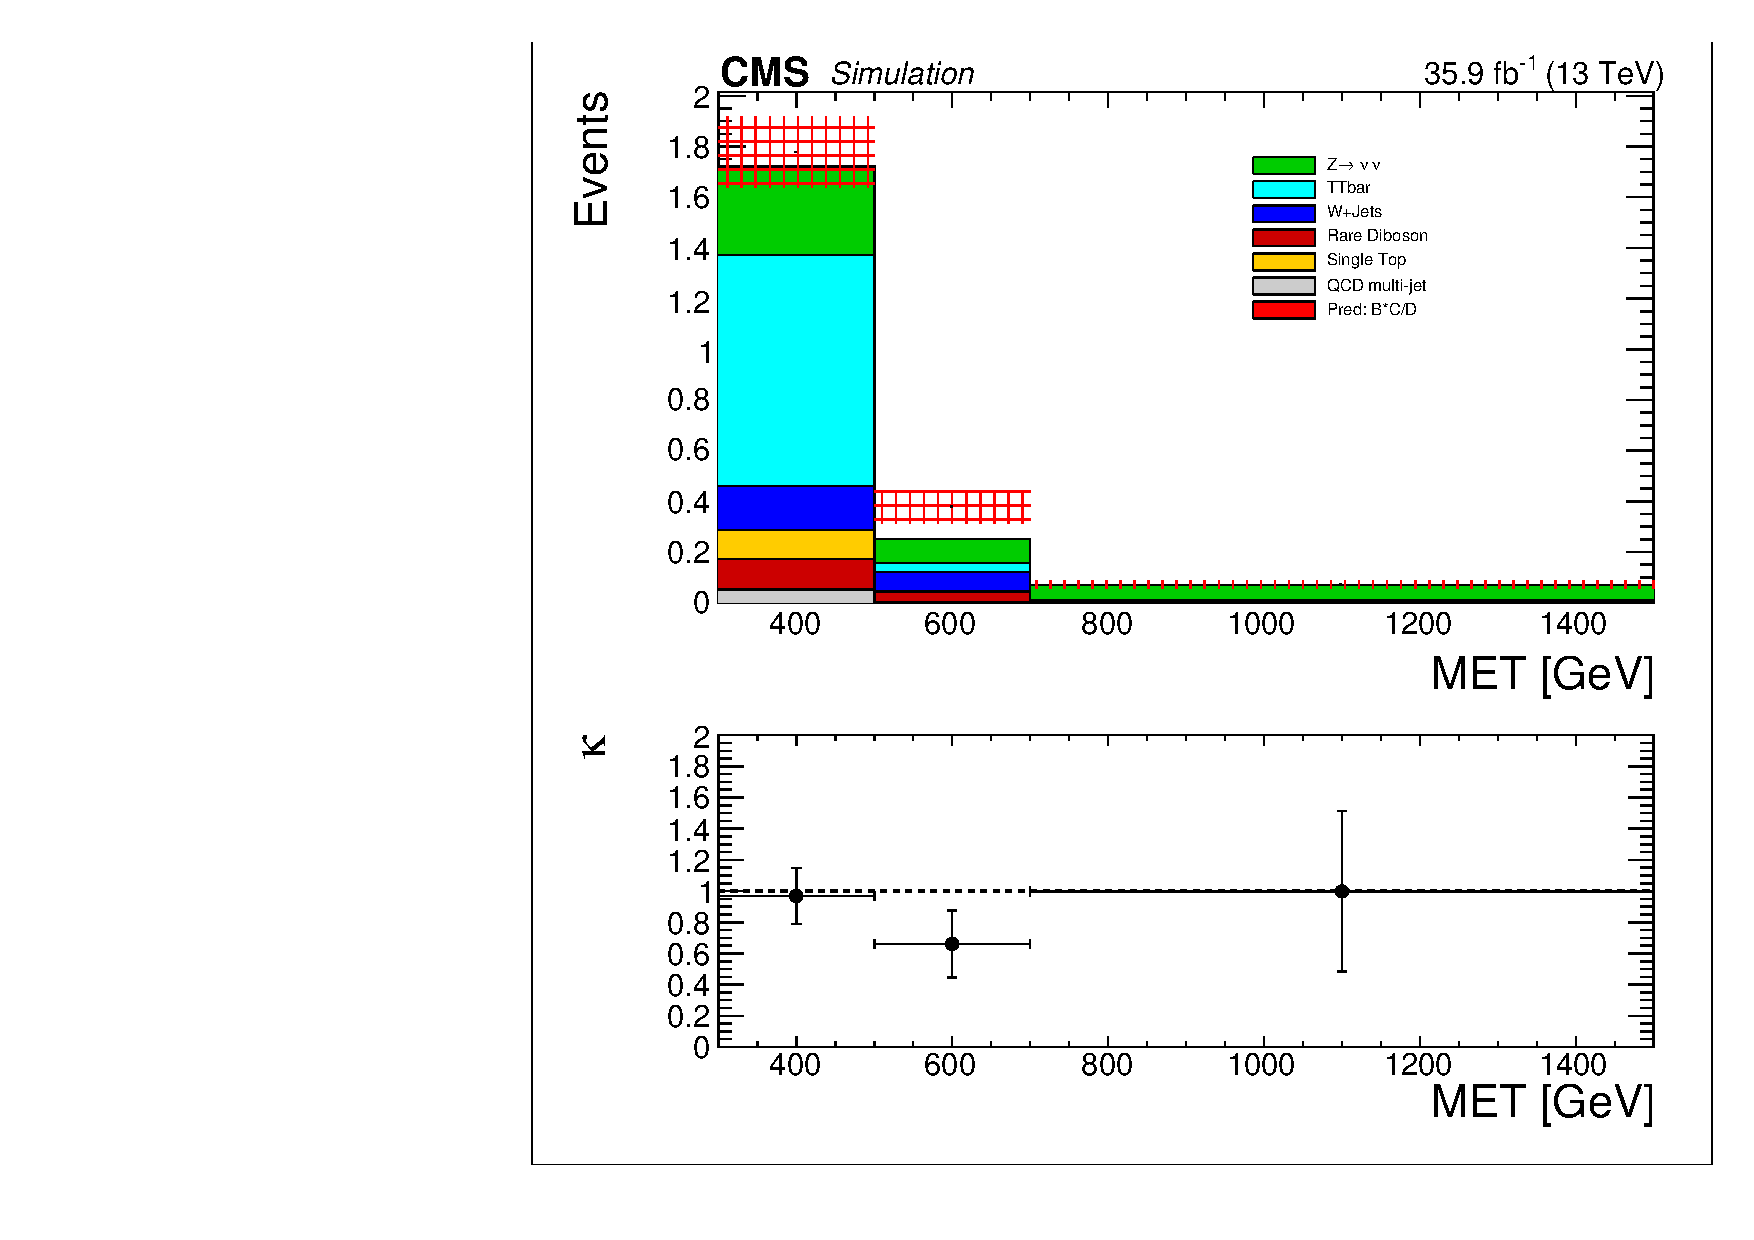
\includegraphics[trim={5px 5px 5px 5px},clip,width=\textwidth]{figs/SUS17006/MCclosure_doubleHiggsRegionTotal.pdf} 
\caption{The double Higgs tag region (A$_{2}$).}
\end{subfigure}
\caption{MET distributions and predictions in the signal regions using simulation only.}
\label{fig:mcclosure}
\end{figure}

\subsection{Study of the SM Background}

We treat the SM backgrounds in the signal region as consisting of three main components:
\begin{itemize}
\item $Z\rightarrow\nu\bar{\nu}$ in which the invisible Z gives true MET (`Z-invisible').
\item Semi-leptonic W or t production in which the lepton is not identified (`lost-lepton').
\item fake MET arising from jet mis-measurement (`QCD'). Typically, the jet $p_{T}$ is underestimated (the thing dont work!).
\end{itemize}

To understand these backgrounds in data, three control regions were defined to serve as a proxy for each source.
\begin{itemize}
\item A single-photon control region, after artificially removing the photon from event reconstruction, closely mimics the Z-invisible background. For high-$p_{T}$, both photons and Z bosons become massless, neutral, gauge bosons whose kinematics are expected to be similar.
\item The single-lepton control region mimics the lost-lepton background.
\item The low-$\Delta\phi$ control region most closely mimics the QCD background.
\end{itemize}

\subsection{Closure of the Estimation Within the Data Control Regions}

As they are orthogonal to our signal regions, we are able to test the closure of the background estimation technique independently in each of the three control regions. By comparing the prediction of the SM yields (using the ABCD method) with those observed in the signal-like bins, the validity of the technique can be verified for that particular background category. The comparisons for the single-photon, single-lepton and low-$\Delta\phi$ control regions can be seen in Figures \ref{fig:closurephoton}, \ref{fig:closuresinglelep}, \ref{fig:closurelowdphi}, respectively. $\kappa$ in bottom panel is defined as the ratio of the prediction to the true event yield (as usual). These comparisons are used for validation of the background estimation technique only, they are not used in the estimation.

\begin{figure}[htbp]
\begin{subfigure}[b]{0.5\textwidth}
\centering
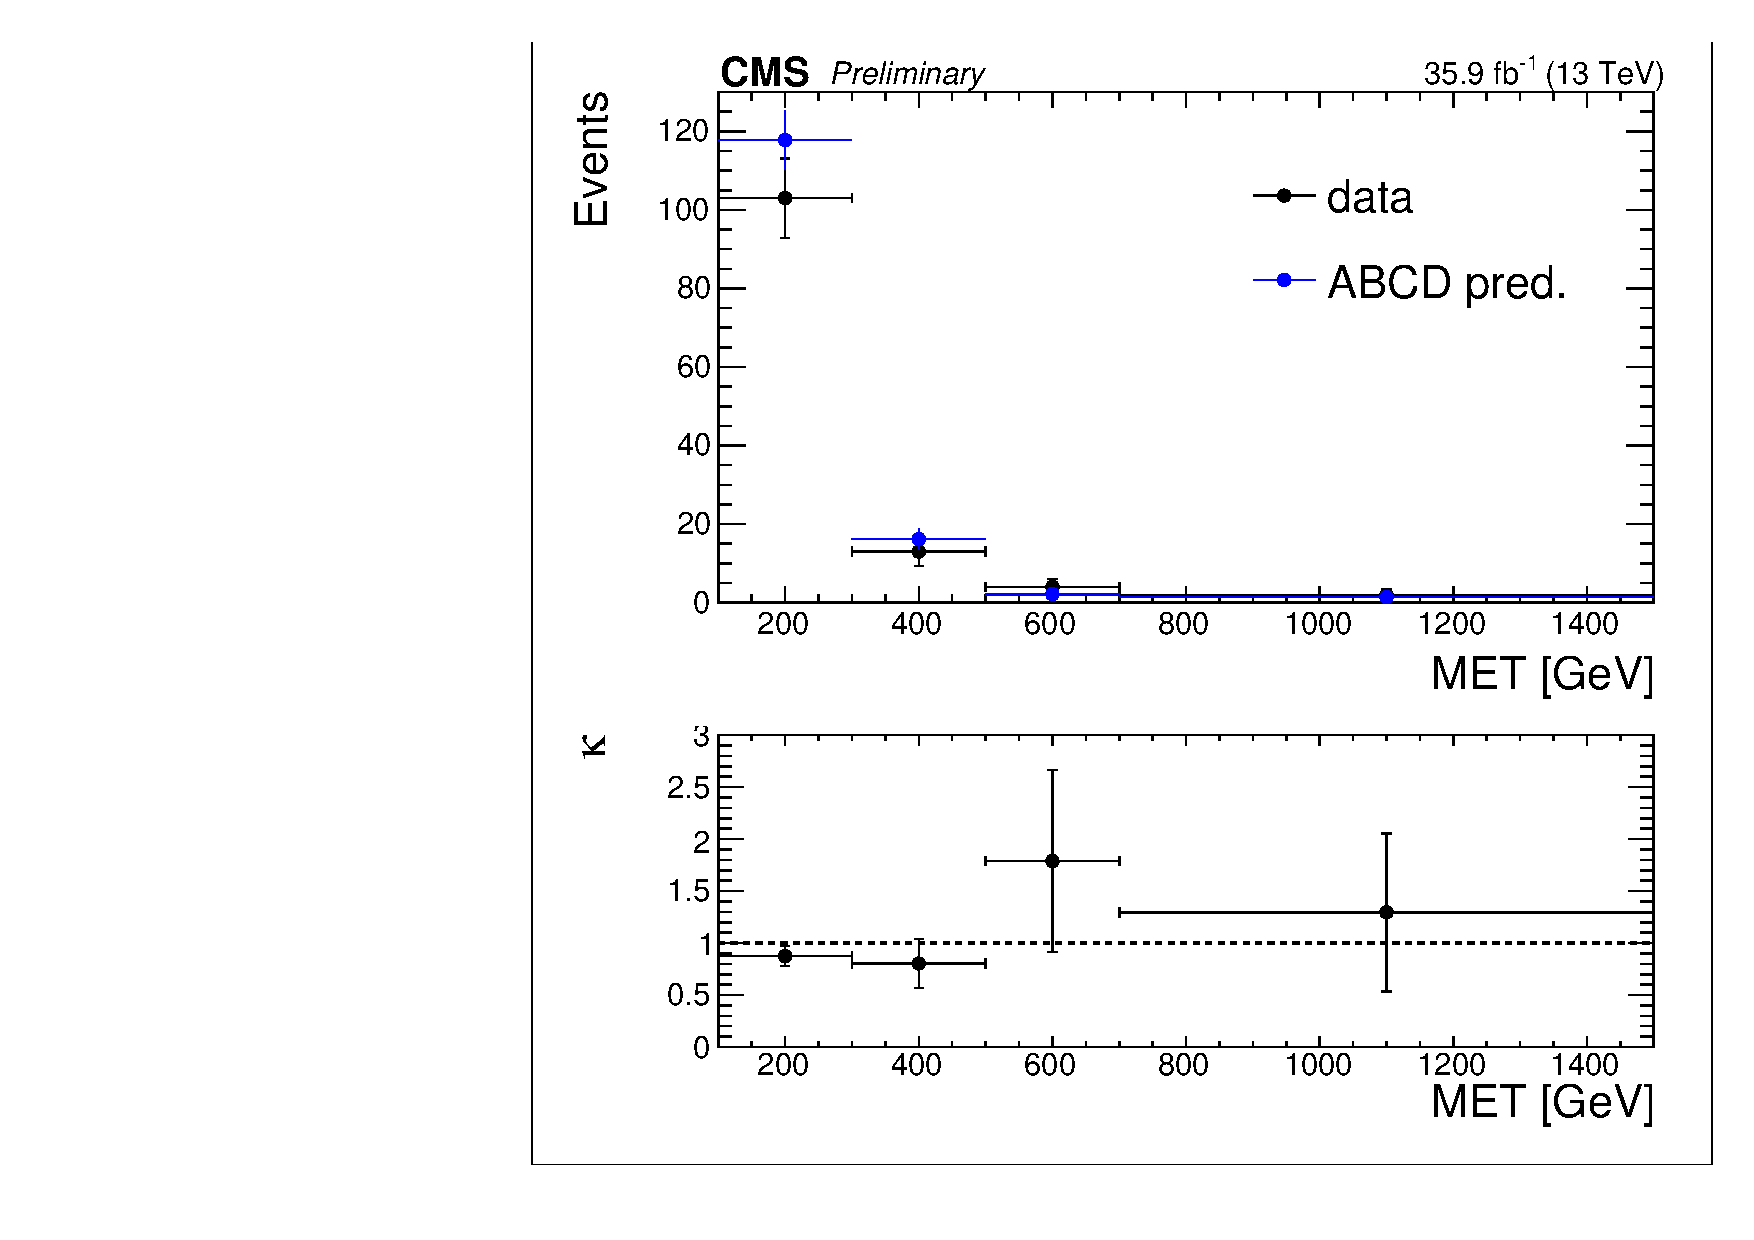
\includegraphics[trim={5px 5px 5px 5px},clip,width=\textwidth]{figs/SUS17006/dataClosure_single-tagSR_photon.pdf}
\caption{The single Higgs tag region (A$_{1}$).}
\end{subfigure}
\begin{subfigure}[b]{0.5\textwidth}
\centering
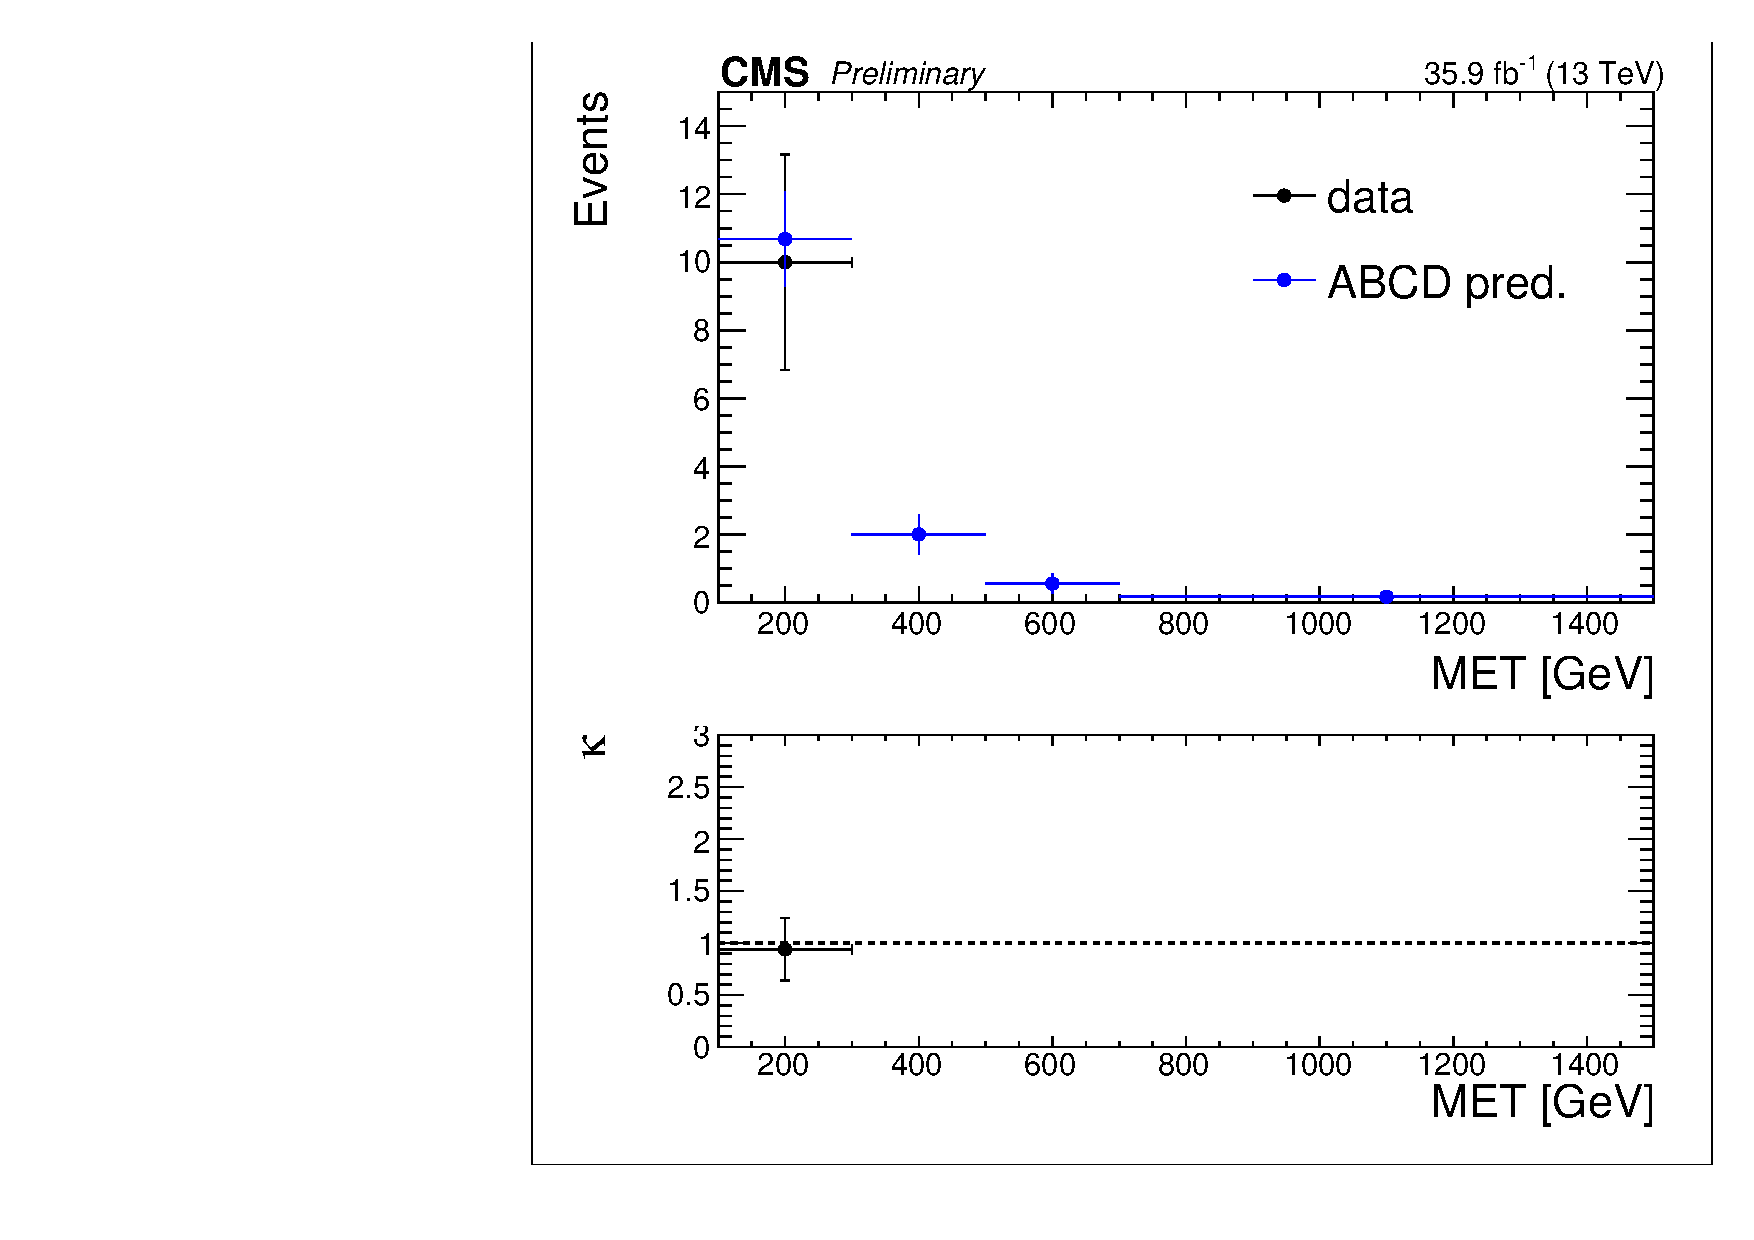
\includegraphics[trim={5px 5px 5px 5px},clip,width=\textwidth]{figs/SUS17006/dataClosure_double-tagSR_photon.pdf} 
\caption{The double Higgs tag region (A$_{2}$).}
\end{subfigure}
\caption{Closure within the single-photon data control region.}
\label{fig:closurephoton}
\end{figure}

\begin{figure}[htbp]
\begin{subfigure}[b]{0.5\textwidth}
\centering
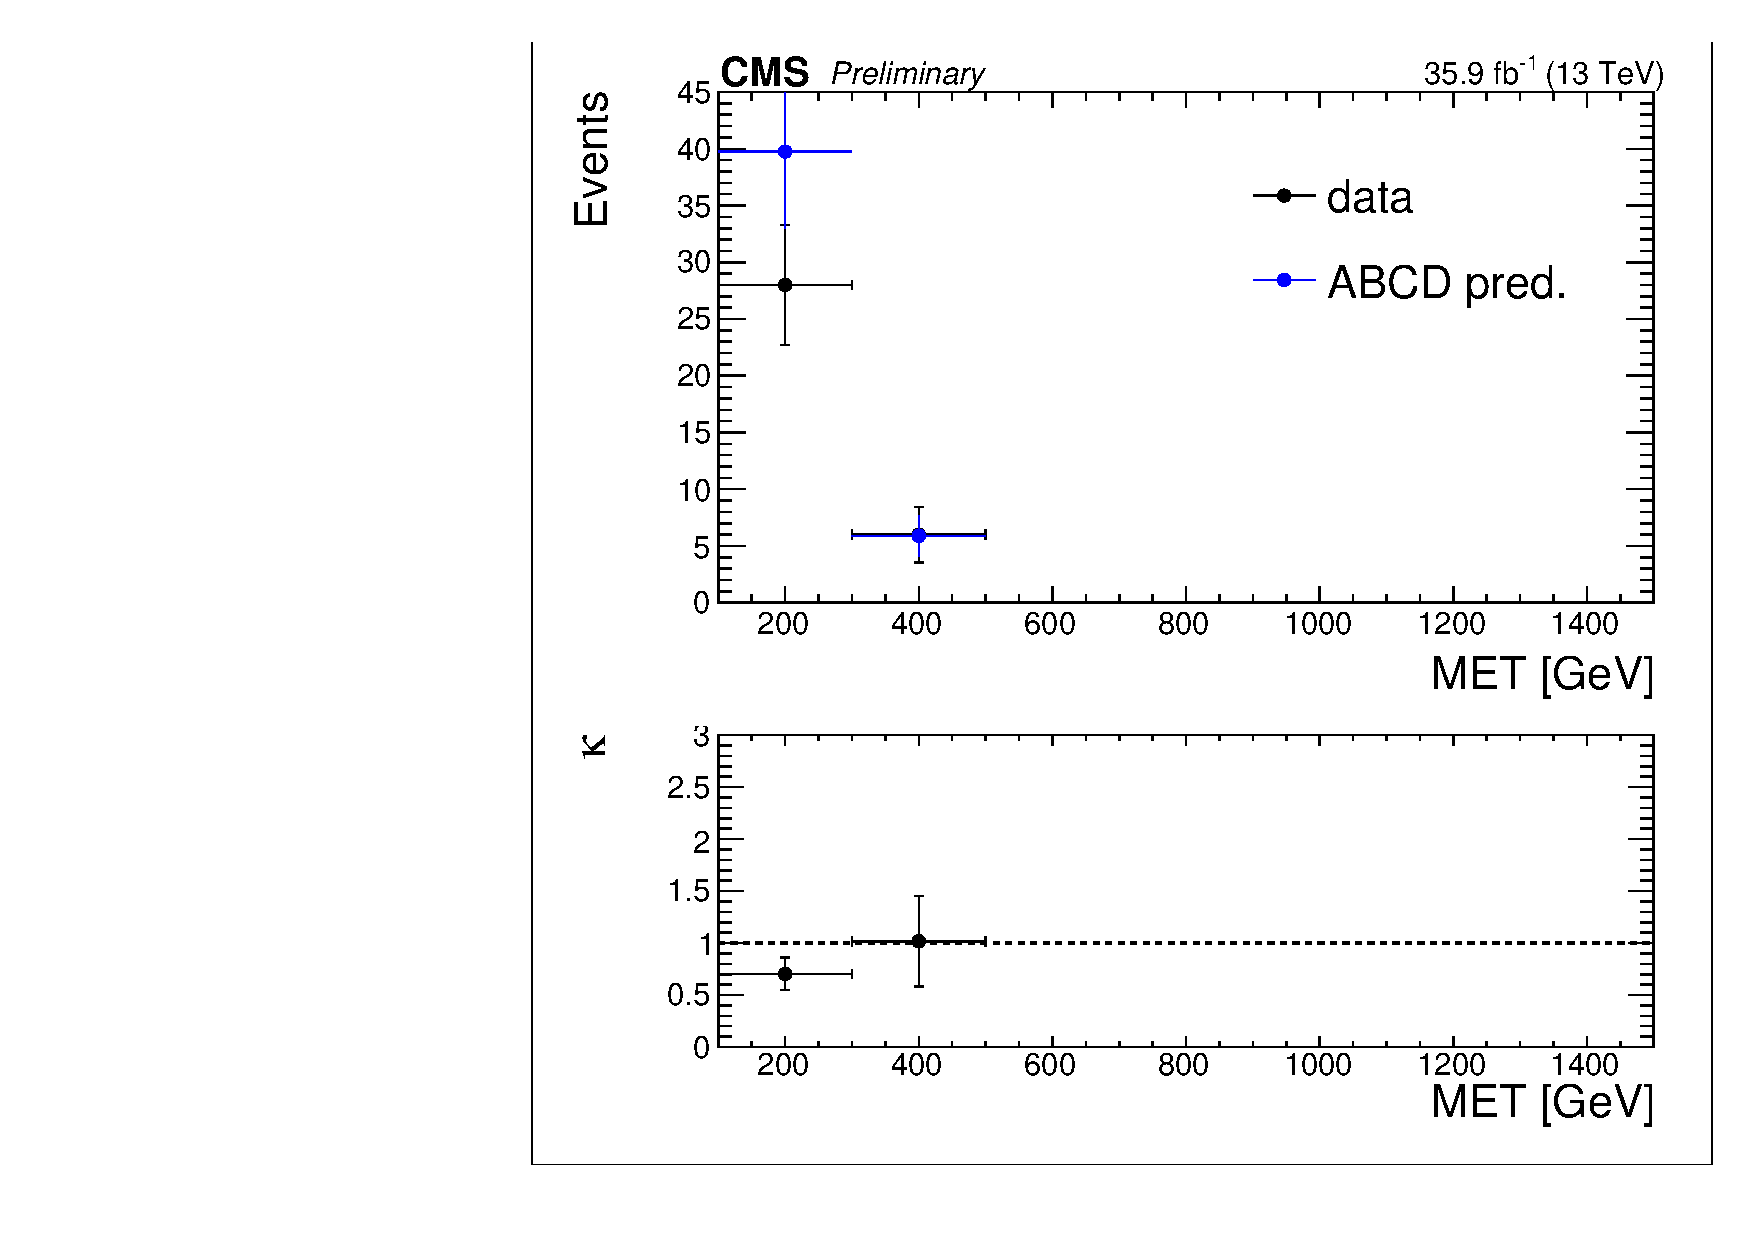
\includegraphics[trim={5px 5px 5px 5px},clip,width=\textwidth]{figs/SUS17006/dataClosure_single-tagSR_singleLep.pdf}
\caption{The single Higgs tag region (A$_{1}$).}
\end{subfigure}
\begin{subfigure}[b]{0.5\textwidth}
\centering
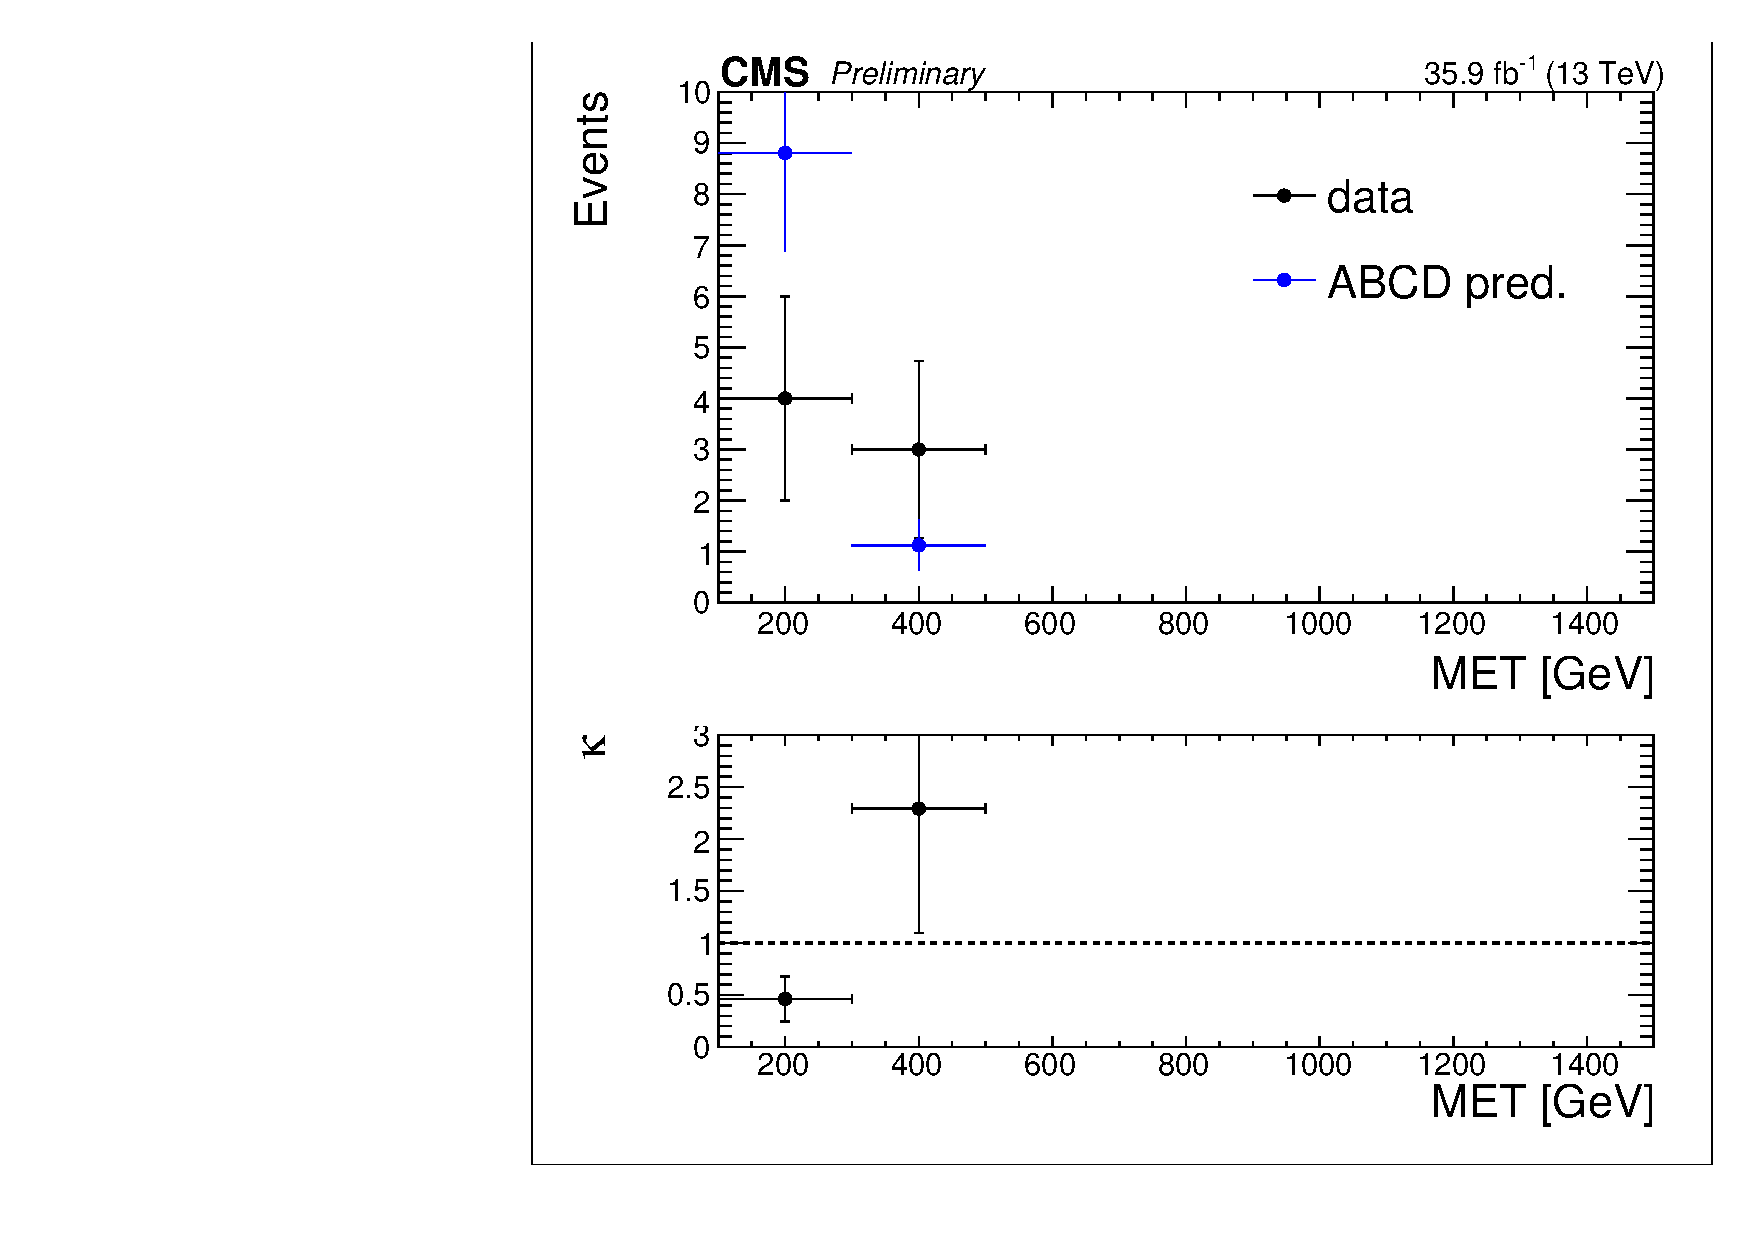
\includegraphics[trim={5px 5px 5px 5px},clip,width=\textwidth]{figs/SUS17006/dataClosure_double-tagSR_singleLep.pdf} 
\caption{The double Higgs tag region (A$_{2}$).}
\end{subfigure}
\caption{Closure within the single-lepton (e, $\mu$) data control region.}
\label{fig:closuresinglelep}
\end{figure}

\begin{figure}[htbp]
\begin{subfigure}[b]{0.5\textwidth}
\centering
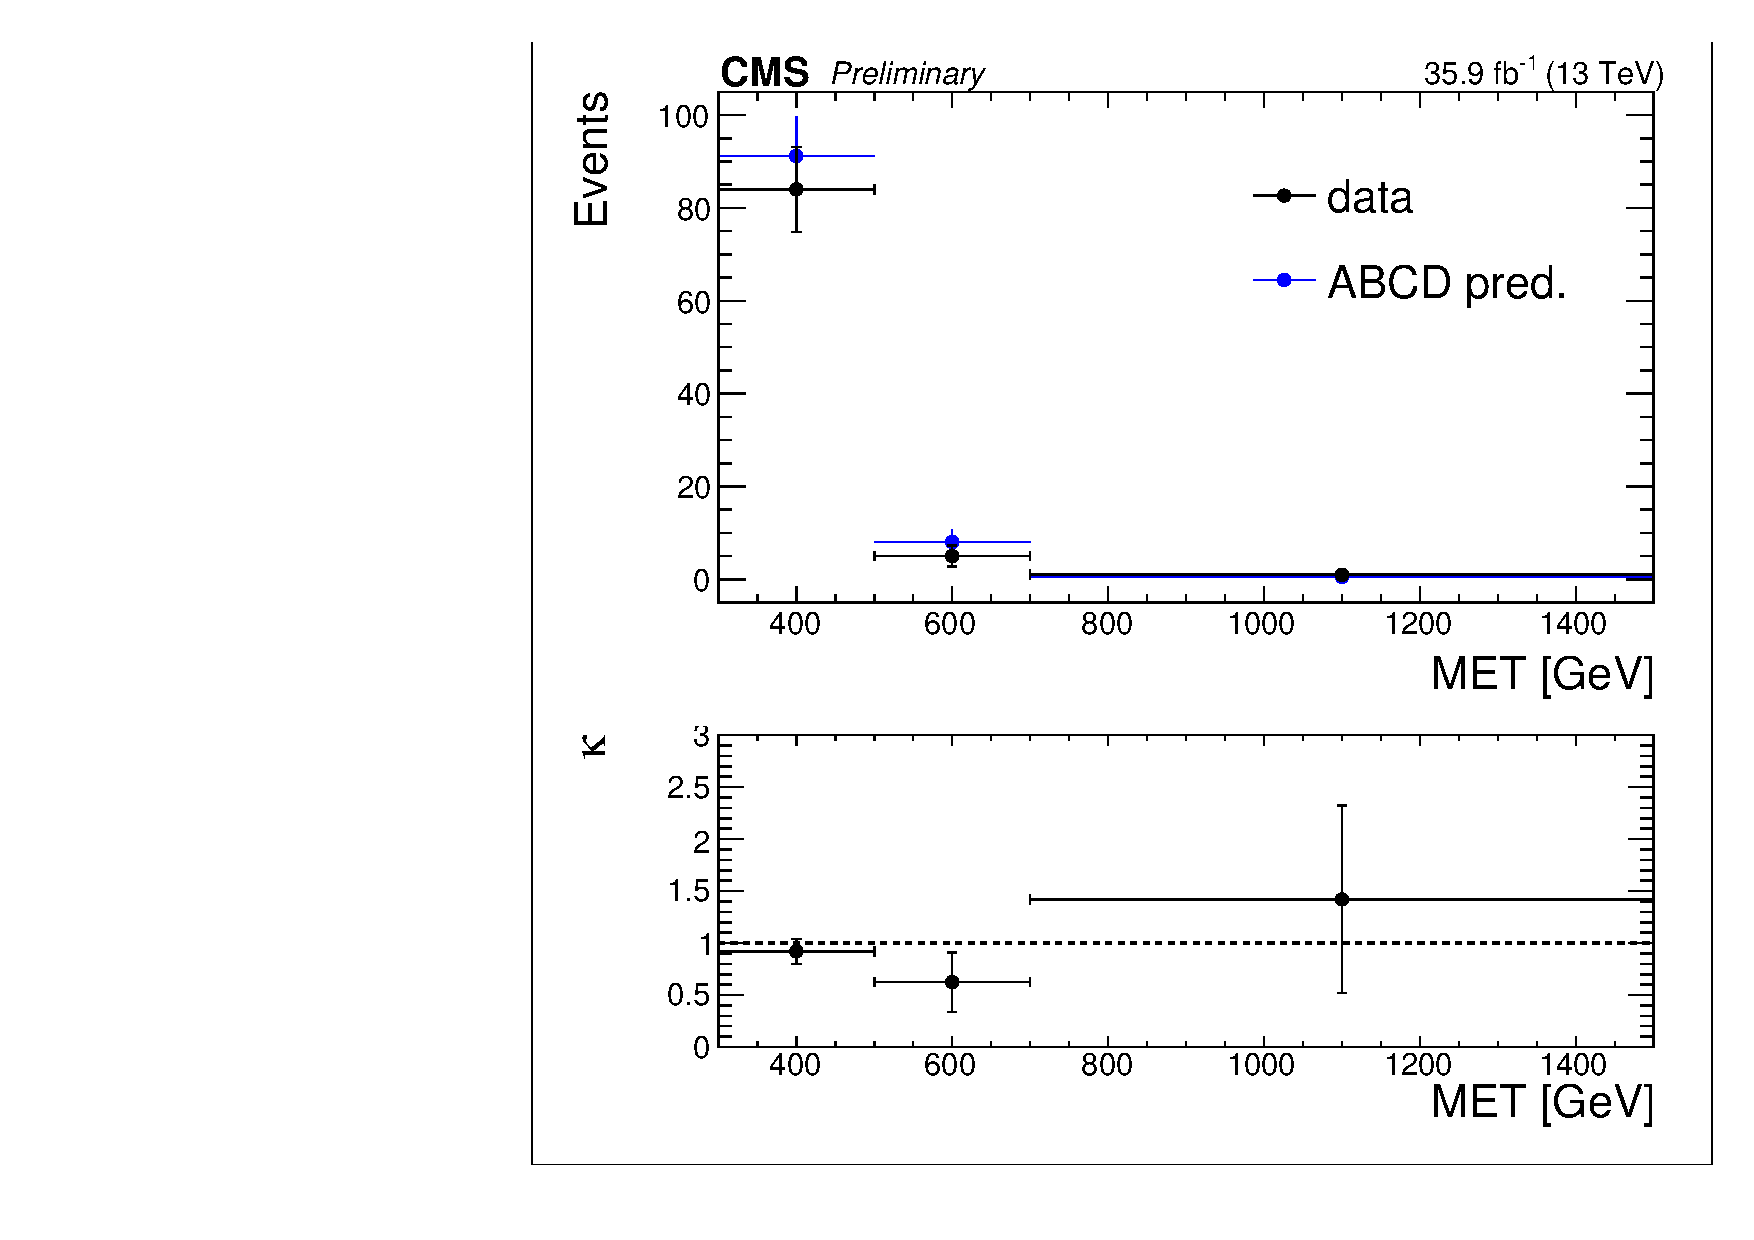
\includegraphics[trim={5px 5px 5px 5px},clip,width=\textwidth]{figs/SUS17006/dataClosure_single-tagSR_lowDphi.pdf}
\caption{The single Higgs tag region (A$_{1}$).}
\end{subfigure}
\begin{subfigure}[b]{0.5\textwidth}
\centering
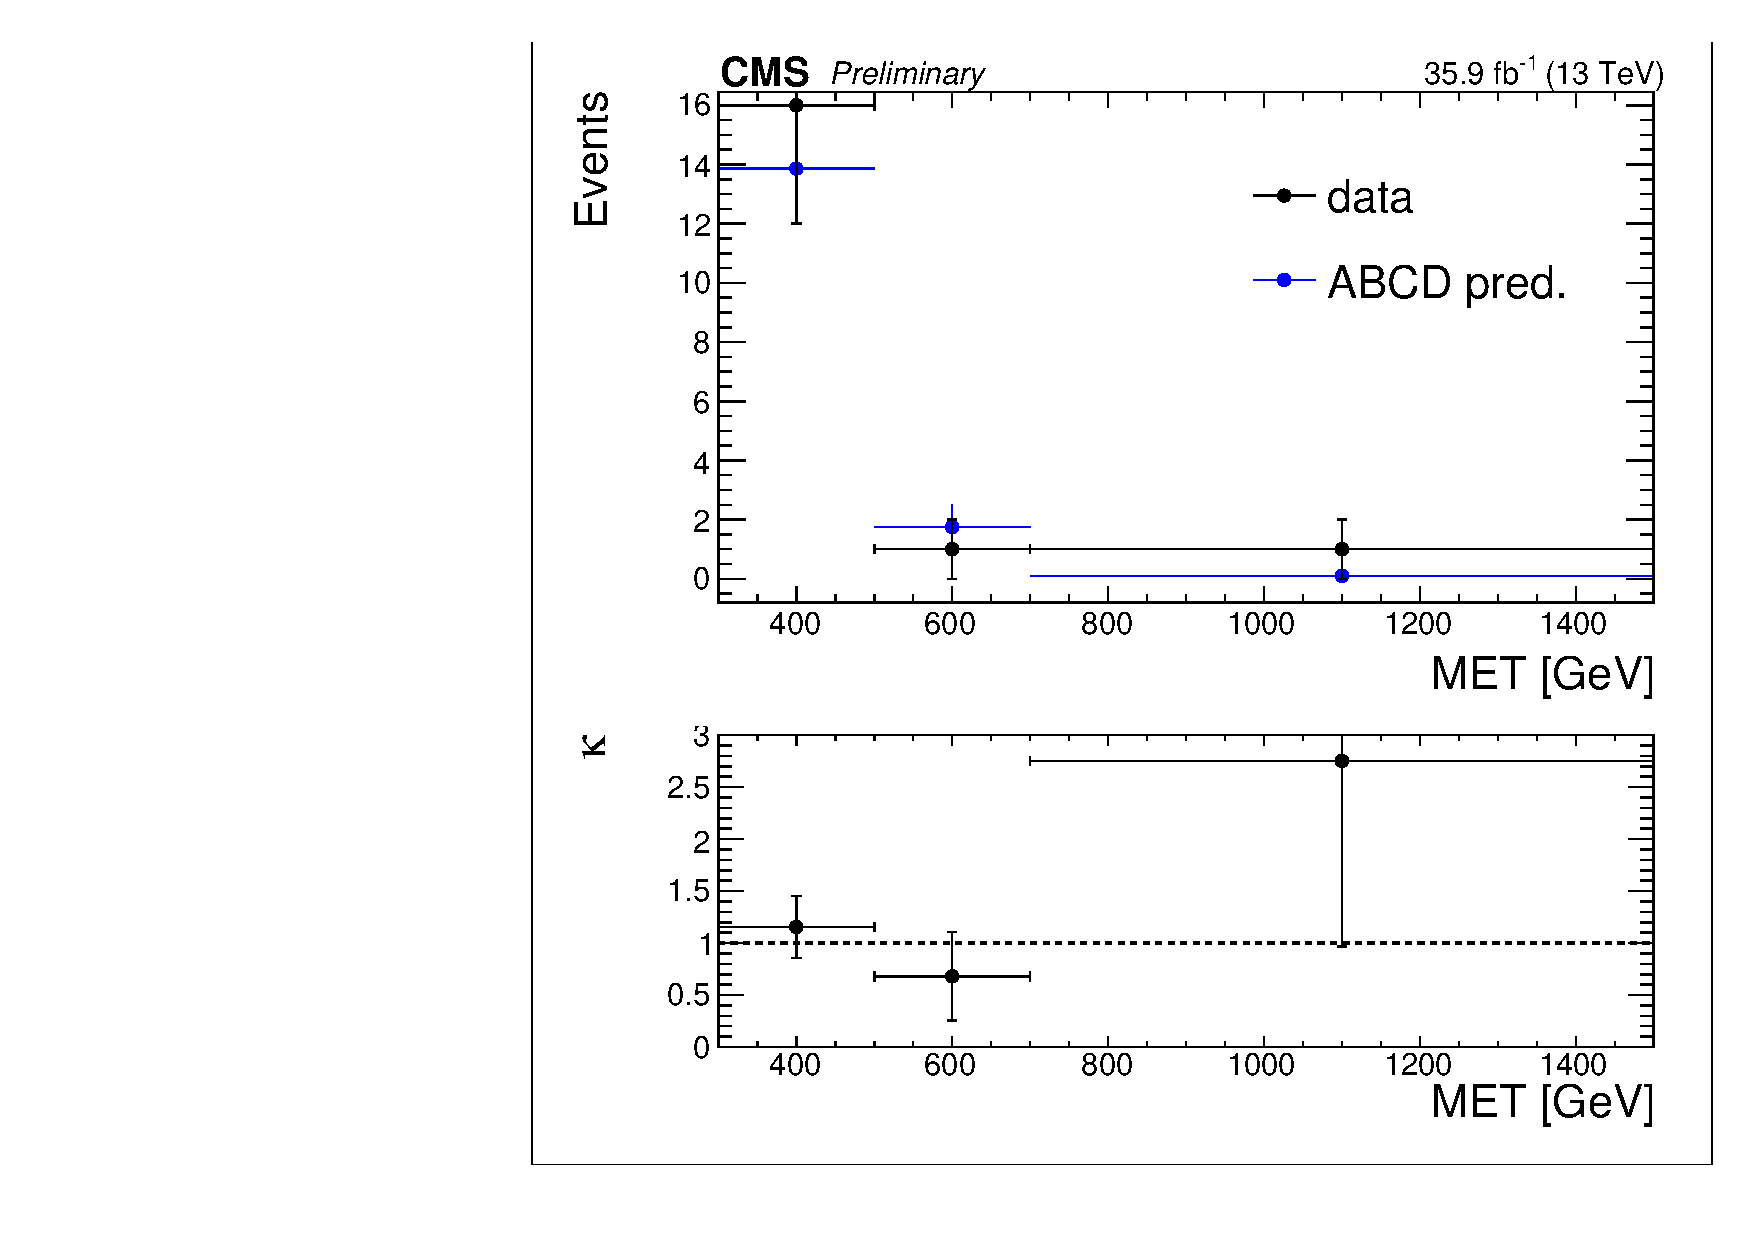
\includegraphics[trim={5px 5px 5px 5px},clip,width=\textwidth]{figs/SUS17006/dataClosure_double-tagSR_lowDphi.pdf} 
\caption{The double Higgs tag region (A$_{2}$).}
\end{subfigure}
\caption{Closure within the low-$\Delta\phi$ data control region.}
\label{fig:closurelowdphi}
\end{figure}

\subsection{$\kappa$ as a Correction to the Estimation}
\label{sec:kappa}

To correct for the observed non-closure of the background estimation method a correction, $\kappa$ is applied to the SM background prediction. $\kappa$ is obtained by dividing the MC yields for the signal region by that predicted: $\kappa  \equiv A_{mc} \,/  \ (B_{mc} \cdot \ (\frac{ C_{mc}} {D_{mc}}\ ) \ )$. There are 2x3=6 values of $\kappa$, one for each signal bin. The corrections are applied as follows: $A_{pred} = B_{obs} \cdot \ (\frac{ C_{obs}} {D_{obs}}\ ) \cdot \kappa$.

Taking into account the information from all the validation regions, we have obtained a set of scale-factors that can be applied to the signal region to test the closure in MC that mimics the data. The dependence of the scale-factors on MET is studied in a looser phase-space with AK8 jet $p_{T}>170\,\textrm{GeV}$. The Low $\Delta\phi$ scale factors show no MET dependence and are determined integrated over MET$>300\,\textrm{GeV}$. The Single-lepton region does show MET dependence. The scale-factors that are determined in MET bins are shown in Table \ref{tab:ScaleFactorMET}. The scale factors derived from each of the validation regions are shown in Table \ref{tab:ScaleFactorVR}. 

These scale factors are then applied directly to the signal region MC to check $\kappa$ with a composition that better reflects the data. Since most of the scale factors are less than one the background decreases in Figure \ref{fig:mcclosure} relative to Figure \ref{fig:mcclosuresf} but still preserves closure so that $\kappa$ is statistically compatible with unity. A distribution of $\kappa$ is derived by throwing gaussian toys for each of the scale factors. We apply the scale factors from each toy to obtain a distribution of $\kappa$.

\begin{table}[htbp!]
\caption{ Summary of the Single Lepton Validation region scale-factors for each of the MET bins in the anti-tag control regions. }
\centering
\begin{tabular}{|c|c|c|}
\hline \hline
\multicolumn{3}{c}{Single Lepton $C_{SF}$}\\
\hline \hline
MET [300,500] & [500,700] & $>700$~GeV\\
$0.47\pm0.05$ & $0.54\pm0.15$ & $0.18\pm 0.1$ \\  \hline\hline
\multicolumn{3}{c}{Single Lepton $D_{SF}$}\\
\hline \hline
$0.49\pm0.02$ & $0.40\pm0.05$ & $0.35\pm 0.08$ \\  \hline
\hline \hline
\end{tabular}
\label{tab:ScaleFactorMET}
\end{table}

\begin{table}
\centering
\caption{Summary of the Validation region scale-factors derived integrated over the MET search bins. They are computed for each of the regions defined at the beginning of the Section.}
\begin{tabular}{c|c|c|c|c|c}
\hline \hline
\multicolumn{6}{c}{Low $\Delta\phi$}\\
\hline \hline
$A^{1H}_{SF}$ & $A^{2H}_{SF}$ & $C_{SF}$ & $B^{1}_{SF}$ & $B^{2}_{SF}$ & $D_{SF}$  \\ \hline
   $1.1 \pm 0.33$ &$0.85 \pm 0.12$&  $0.93 \pm 0.1$ & $0.88 \pm 0.04$ & $1.2 \pm 0.16$  & $0.71 \pm 0.027$ \\ \hline
\hline \hline
\multicolumn{6}{c}{Single Lepton}\\
\hline \hline
$A^{1H}_{SF}$ & $A^{2H}_{SF}$ & $C_{SF}$ & $B^{1}_{SF}$ & $B^{2}_{SF}$ & $D_{SF}$  \\ \hline
   %$0.63 \pm 0.069$ & $0.64 \pm 0.15$  & \MET dependent &   $0.65 \pm 0.1$ & $0.71 \pm 0.059$  & \MET dependent\\ \hline
   %$0.64 \pm 0.033$ & $0.68 \pm 0.068$  & \MET dependent &   $0.63 \pm 0.011$ & $0.72 \pm 0.023$  & \MET dependent\\ \hline
   $0.61\pm 0.04$ & $0.59\pm0.08$ & MET dependent &  $0.59\pm 0.016$ & $0.71\pm 0.04$  & MET dependent\\ \hline
\hline \hline
\multicolumn{6}{c}{Photon}\\
\hline \hline
$A^{1H}_{SF}$ & $A^{2H}_{SF}$ & $C_{SF}$ & $B^{1}_{SF}$ & $B^{2}_{SF}$ & $D_{SF}$ \\ \hline
   $0.61 \pm 0.088$ & $0.75 \pm 0.29$ & $0.5 \pm 0.07$ & $0.98 \pm 0.094$ & $2.58 \pm 0.63$ & $0.71 \pm 0.035$\\ \hline
\end{tabular}
\label{tab:ScaleFactorVR}
\end{table}

Figure \ref{fig:mcclosuresf} shows the modified MET distributions in the 6 signal regions after correcting simulation with the scale factors derived from the data control regions.

\begin{figure}[htbp]
\begin{subfigure}[b]{0.5\textwidth}
\centering
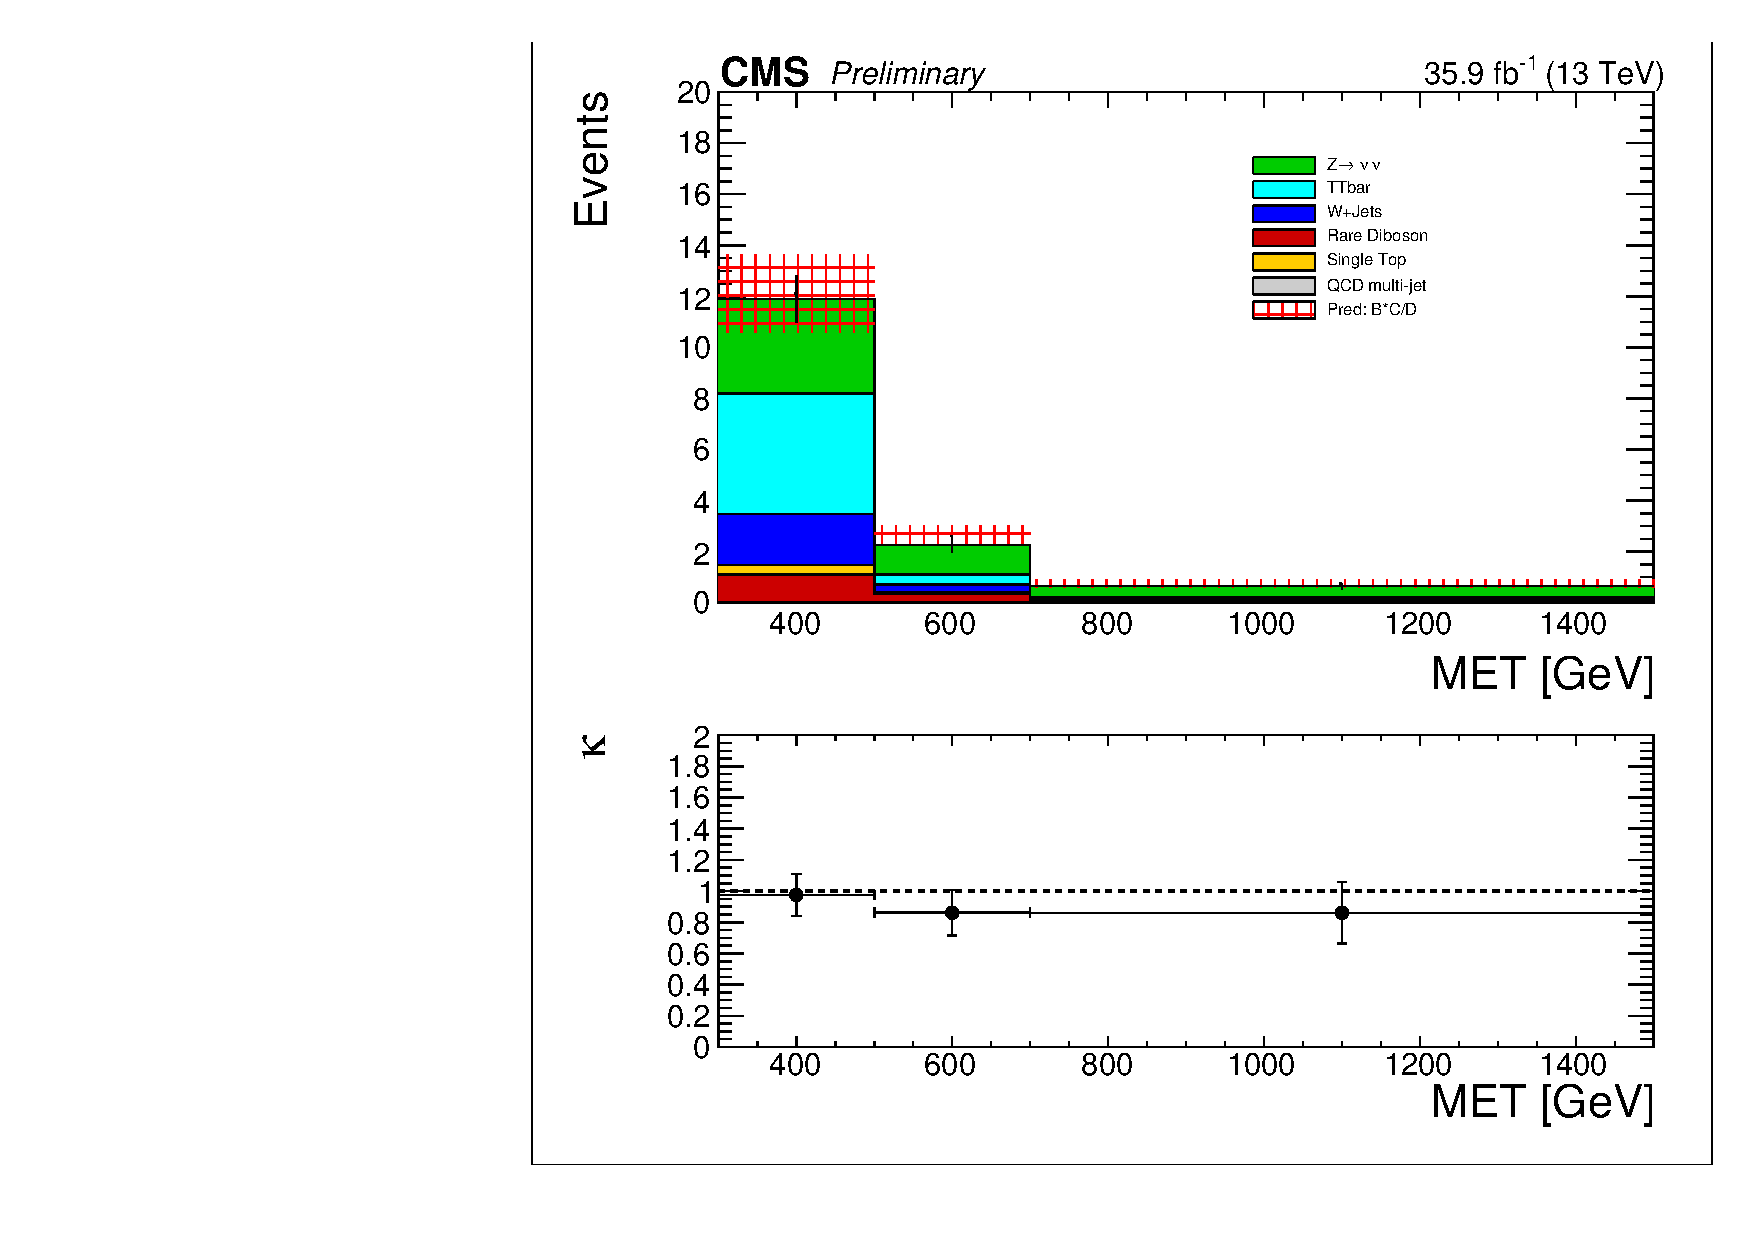
\includegraphics[trim={5px 5px 5px 5px},clip,width=\textwidth]{figs/SUS17006/MCclosureSF_singleHiggsRegionTotal.pdf}
\caption{The single Higgs tag region (A$_{1}$).}
\end{subfigure}
\begin{subfigure}[b]{0.5\textwidth}
\centering
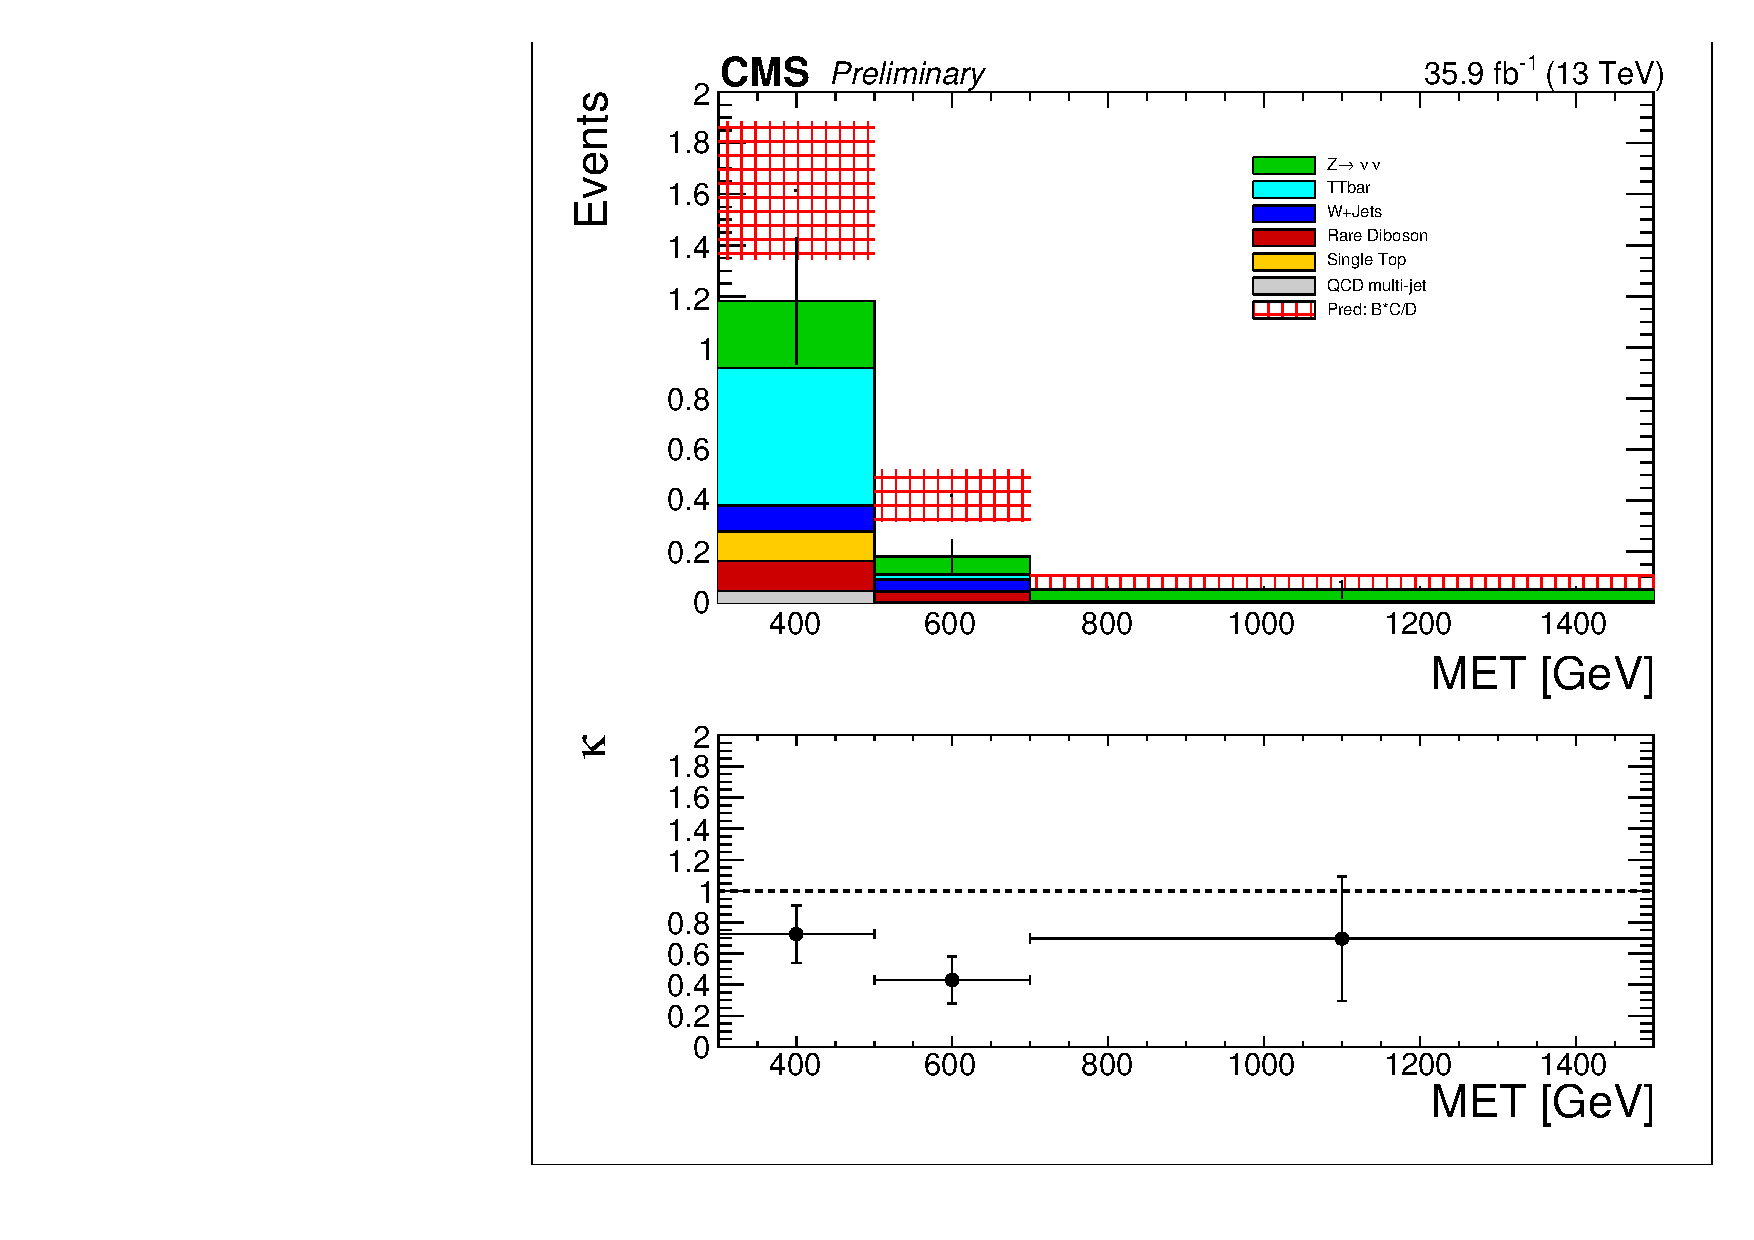
\includegraphics[trim={5px 5px 5px 5px},clip,width=\textwidth]{figs/SUS17006/MCclosureSF_doubleHiggsRegionTotal.pdf} 
\caption{The double Higgs tag region (A$_{2}$).}
\end{subfigure}
\caption{MET distributions and the predictions in the signal regions using simulation with scale factors from data.}
\label{fig:mcclosuresf}
\end{figure}

\subsection{Sideband Yields \& Predictions}

Observed yields in data for the 4x3=12 sideband regions (e.g. B, C, D in Figure \ref{fig:abcd}) are seen in Table \ref{tab:sidebandyields}, alongside the prediction and $\kappa$ for each signal bin.

\begin{table}[htbp]
\centering
\caption{Yields in each of the 6 analysis regions.}
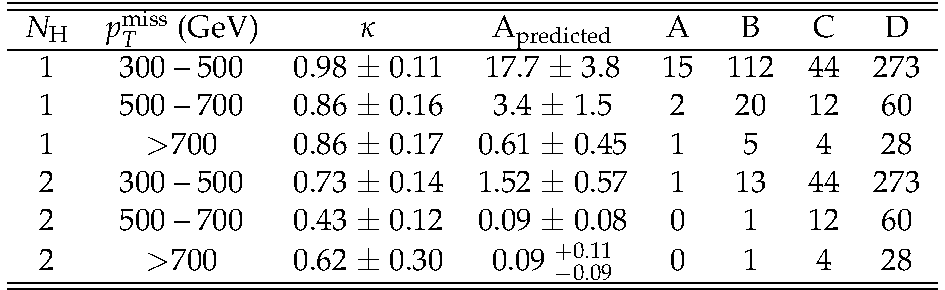
\includegraphics[width=0.75\textwidth]{figs/SUS17006/CMS-SUS-17-006_Table-aux_001.pdf}
\label{tab:sidebandyields}
\end{table}

\input signal-systematics.tex

\section{Yields in the Signal Regions and Exclusion Curves}
\label{sec:results}

After unblinding the 4x3=12 sideband regions and performing the background estimation the 2x3=6 signal regions were unblinded. The observed yields, along with the SM background predictions, are seen in Table \ref{tab:DataPred}. Our signal region yields are consistent with the SM background expectation. Additionally, Table \ref{tab:DataPred} shows the expected signal yields for two model points corresponding to gluino $\tilde{g}$ masses of 2000 or 1800 GeV; the mass of the neutralino $\tilde{\chi}_{1}^{0}$ is fixed at 1 GeV; the mass splitting between the gluino $\tilde{g}$ and neutralino $\tilde{\chi}_{2}^{0}$ is fixed at 50 GeV.

\begin{table}[htbp!]
\caption{Signal yields and SM background predictions}
\centering
\begin{tabular}{c|c|c|c|c||c|c|}
\hline \hline
MET bin & ABCD Pred & $\kappa$ & Total Pred. & Obs. & T5HH(2000) & T5HZ(1800) \\
\hline \hline
\multicolumn{7}{c}{1-Higgs Tag} \\ \hline \hline
MET [300,500] & $18.05 \pm 3.39$  & $0.98 \pm 0.11$ & $17.68 \pm 3.85$ & 15 & 0.24 & 0.75  \\ \hline
MET [500,700] & $4 \pm 1.54$ & $0.86 \pm 0.16$ & $3.44\pm 1.47$ &  2  & 0.32 & 0.98 \\\hline
MET $>$ 700 &  $0.71 \pm 0.50$  &  $0.86 \pm 0.17$ & $0.61\pm 0.45$ &  1 & 2.13 & 4.34\\\hline \hline
\multicolumn{7}{c}{2-Higgs Tag} \\  \hline \hline
MET [300,500] &   $2.09 \pm 0.67$  & $0.73 \pm 0.14$ & $1.52 \pm 0.57$ & 1 & 0.17 & 0.35\\ \hline
MET [500,700] & $ 0.2 \pm 0.20$ & $0.43 \pm 0.12$ &$0.09^{+0.08}_{-0.08}$ & 0 & 0.23 & 0.44\\ \hline
MET $>$ 700 & $0.14 \pm 0.16$ & $0.62 \pm 0.30$ & $0.09^{+0.11}_{-0.09}$ & 0 & 1.36 & 1.98\\ \hline
\hline
\end{tabular}
\label{tab:DataPred}
\end{table}

%A visual representation of the single event in the double-H tagged signal bin is seen in Figure \ref{fig:fireworks}.
%\begin{table}[htbp]
%\centering
%\caption{The single double-H tagged event.}
%\includegraphics[width=0.75\textwidth]{figs/SUS17006/fireworks.pdf}
%\label{fig:fireworks}
%\end{table}

Interpreting our results in the context of the T5HH or T5ZH models, the absence of signal allows us to place lower limits on the mass of the gluino $\tilde{g}$. For the statistical treatment, we use the Higgs combination tool to encode the ABCD approach in the likelihood. In this approach, the data card for one search bin contains the observed number of events and the expected signal and background in each of the ABCD regions. A likelihood function is built that contains these ABCD regions and explicitly encodes the relation $A=\kappa B \frac{C}{D}$ and a Gaussian nuisance is assigned for the uncertainty on $\kappa$. The likelihood for each search bin can be described by:

\begin{equation}
\mathcal{L}=\prod^{ABCD}_{i} Poisson\left(n_i \vert bkg_i + r\cdot sig_i\right) \times \prod^{nuisances}_j Constraints\left(\theta_j , \hat{\theta}_j\right)
\end{equation}

where the 4 regions are modeled by Poisson distribution and the term Constraints refers to either Gaussian distributions for the $\kappa$ uncertainties or log normal distributions that model the signal systematics. The expected and observed limits are then calculated based on the asymptotic approximation of the profile likelihood ratio using the CLs criterion to place limits at the $95\%$ confidence level. These exclusion curves are seen in Figure \ref{fig:brazil}. We are able to place lower limits at 95\% confidence level on the gluino $\tilde{g}$ mass at 2010 and 1825 GeV for the T5HH and T5ZH models, respectively. The weaker limit for the T5ZH model is due to the smaller branching fraction of the Z boson to b-quarks and our choice of signal mass window not being optimal for Z reconstruction.

\begin{figure}[htbp]
\centering
\begin{subfigure}[b]{0.45\textwidth}
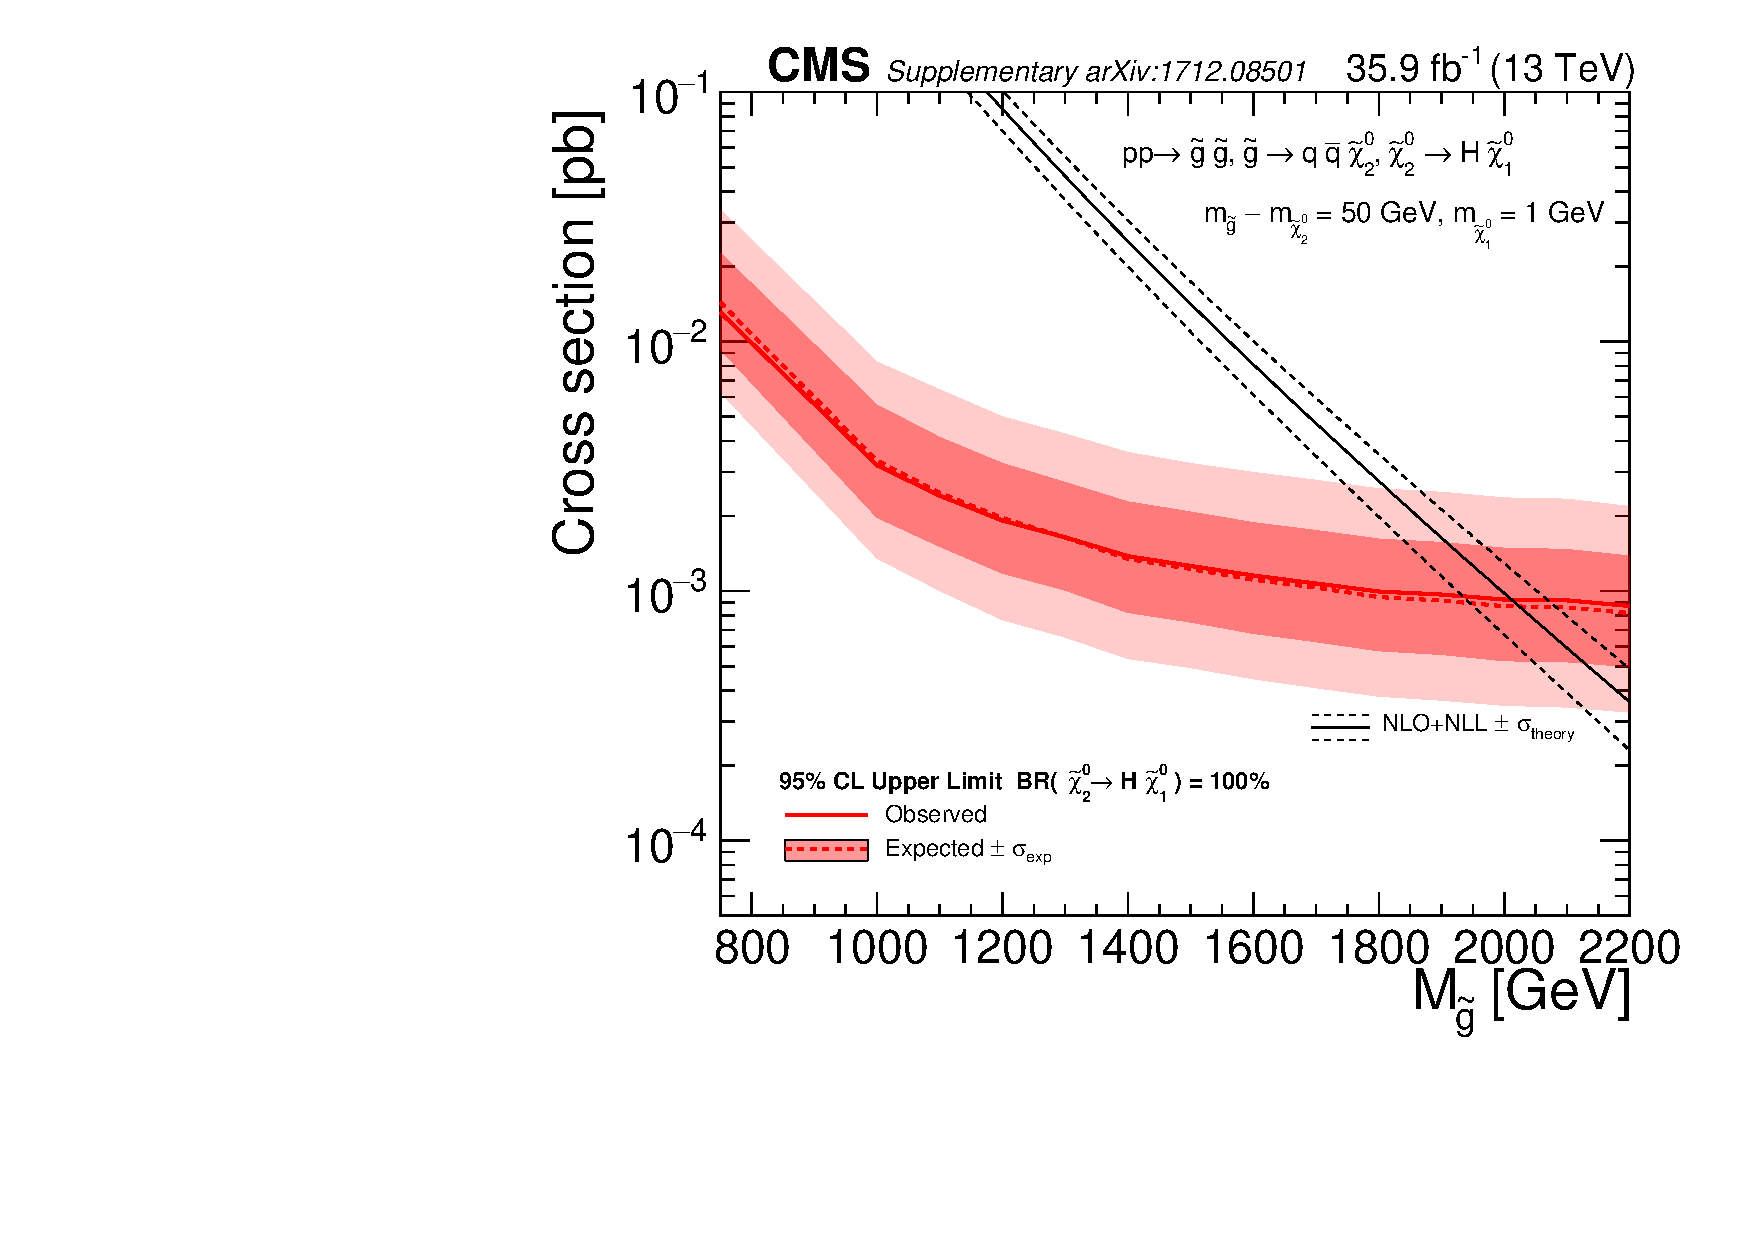
\includegraphics[width=\textwidth]{figs/SUS17006/brazilT5HHResults.pdf}
\caption{T5HH}
\end{subfigure}
\begin{subfigure}[b]{0.45\textwidth}
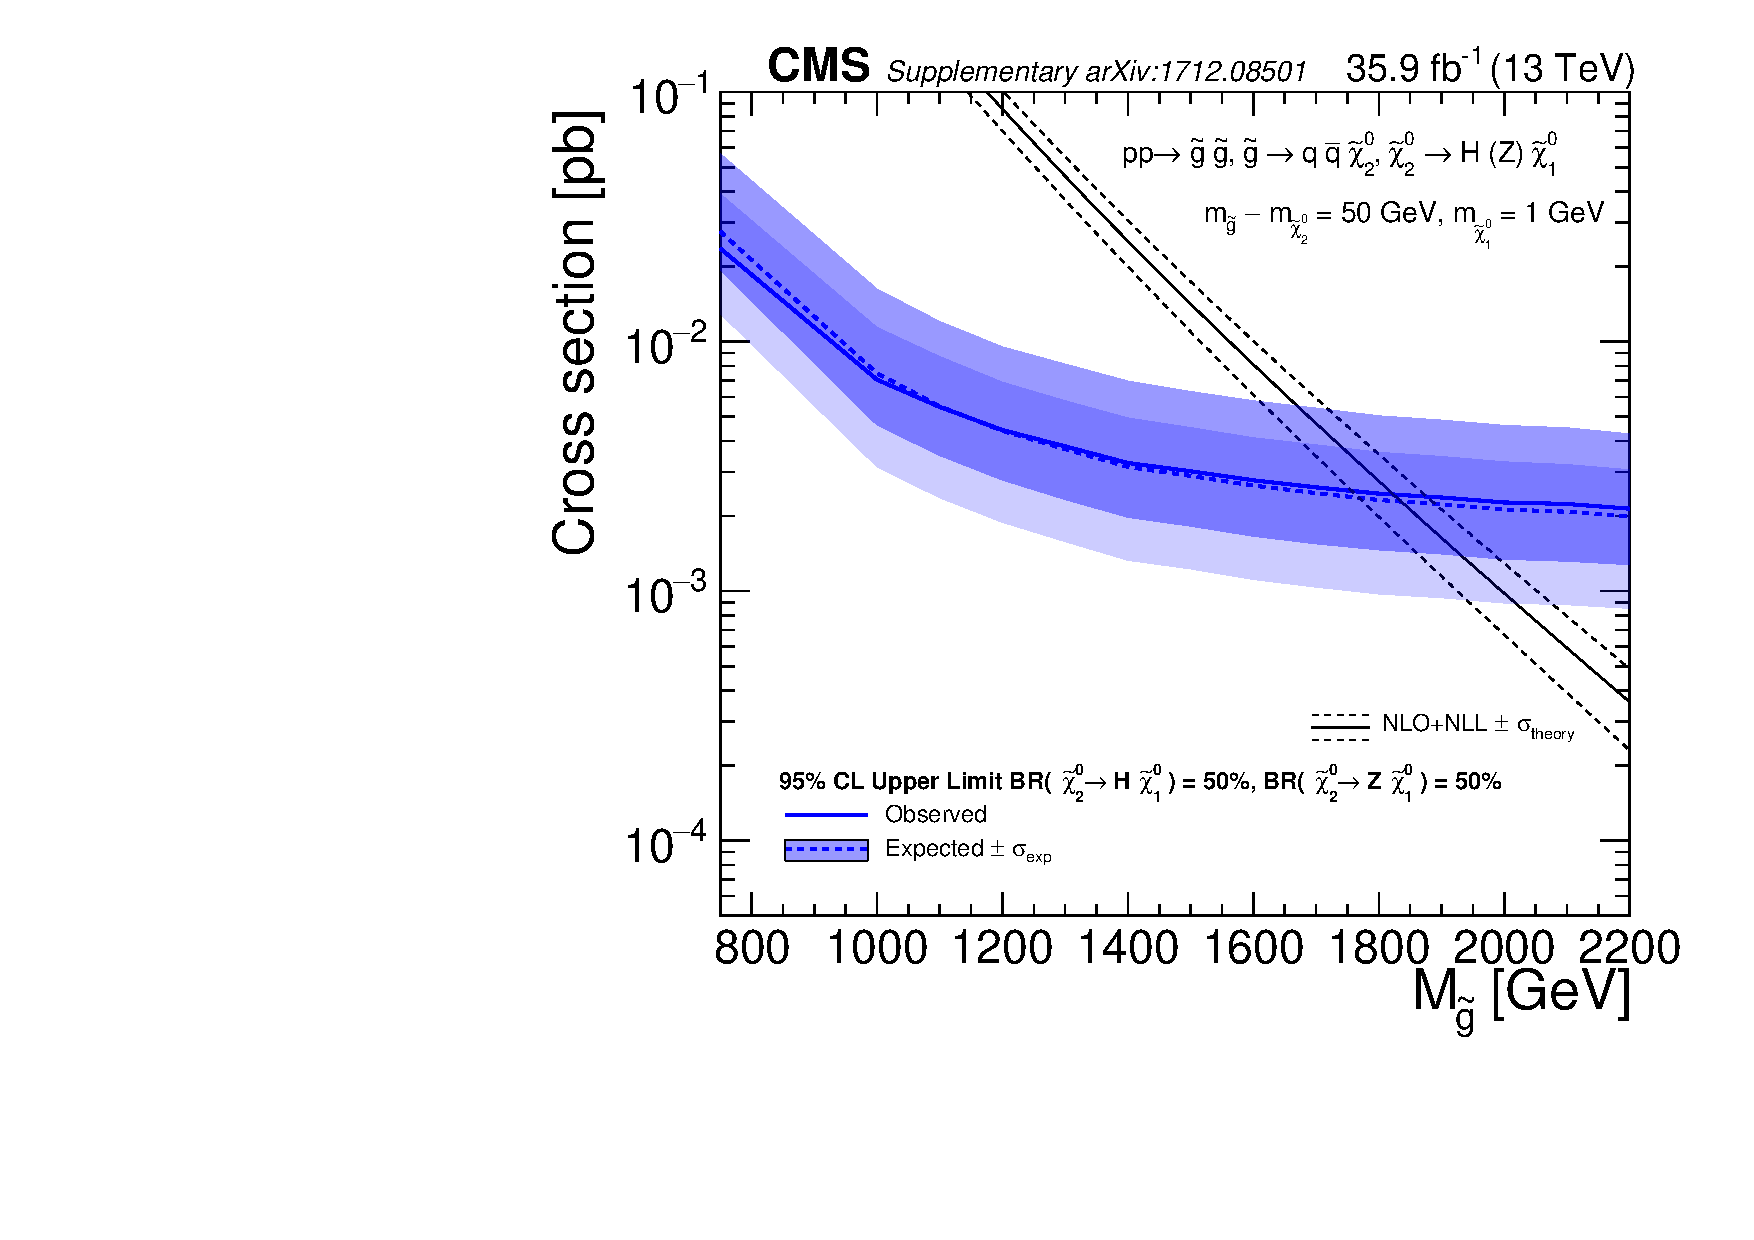
\includegraphics[width=\textwidth]{figs/SUS17006/brazilT5HZResults.pdf}
\caption{T5ZH}
\end{subfigure}
\caption{Observed and expected limits on the gluino cross section.}
\label{fig:brazil}
\end{figure}

\section{Reinterpretation}

In Section \ref{sec:results} our results were presented in the context of limit-setting for the T5HH and T5ZH models. Many such SMS models exist within the MSSM which predict the production of high-$p_{T}$ bosons and it is therefore important to include information necessary to make predictions of yields for different final states. This is aided by providing the user with efficiencies for \bbbar-tagging and mass-tagging efficiencies of the AK8 jets. Tagging efficiencies for the three largest decay channels for the H boson are seen in \ref{fig:effH}. Tagging efficiencies for the Z boson are seen in Figure \ref{fig:effZ}, the much lower mass-tagging efficiency for the Z is due to our choice of signal mass window [85, 135 GeV] not being optimal for Z boson reconstruction. These are used to calculate the expected yields in the 6 analysis regions when performing a reinterpretation of the analysis using different final states.

For each event, the yield in each bin can be predicted by first forming the following weights using the tagging efficiencies for the leading two jets, as seen below.

\begin{itemize}
\item double mass tag weight = jet$_{0}\_$signalmass * jet$_{1}\_$signalmass
\item anti mass tag weight = (jet$_{0}\_$sidebandmass * jet$_{1}\_$signalmass) + (jet$_{0}\_$signalmass * jet$_{1}\_$sidebandmass) + (jet$_{0}\_$sidebandmass * jet$_{1}\_$sidebandmass);
\item double bb tag weight = jet$_{0}\_$bbtag * jet$_{1}\_$bbtag;
\item single bb tag weight = (jet$_{0}\_$bbtag * (1-jet$_{1}\_$bbtag)) + ((1-jet$_{0}\_$bbtag)*jet$_{1}\_$bbtag);
\item anti bb tag weight = (1-jet$_{0}\_$bbtag) * (1-jet$_{1}\_$bbtag)
\end{itemize}

These weights are then combined in the following manner to determine the yields across each of the 6 bins for a single event.

\begin{itemize}
\item A1 weight = (single bb tag weight) * (double mass tag weight)
\item A2 weight = (double bb tag weight) * (double mass tag weight)
\item B1 weight = (single bb tag weight) * (anti mass tag weight)
\item B2 weight = (double bb tag weight) * (anti mass tag weight)
\item C weight = (anti bb tag weight) * (double mass tag weight)
\item D weight = (anti bb tag weight) * (anti mass tag weight)
\end{itemize}

Following this prescription, the authors found that the largest deficit was in the D region, with a difference of -36\% difference from nominal, as seen in Table \ref{tab:predclos}.
The greatest over-prediction is found in the B2 region, with a surplus of +8.2\% events relative to nominal.
The closure in the other bins fall somewhere in this range.
As a cross-check to your yield estimates, consult Table \ref{tab:sigeff} which shows the true signal event efficiencies for the T5qqqqHH model with a gluino mass of 2200 GeV.

\clearpage

\begin{figure}
\centering
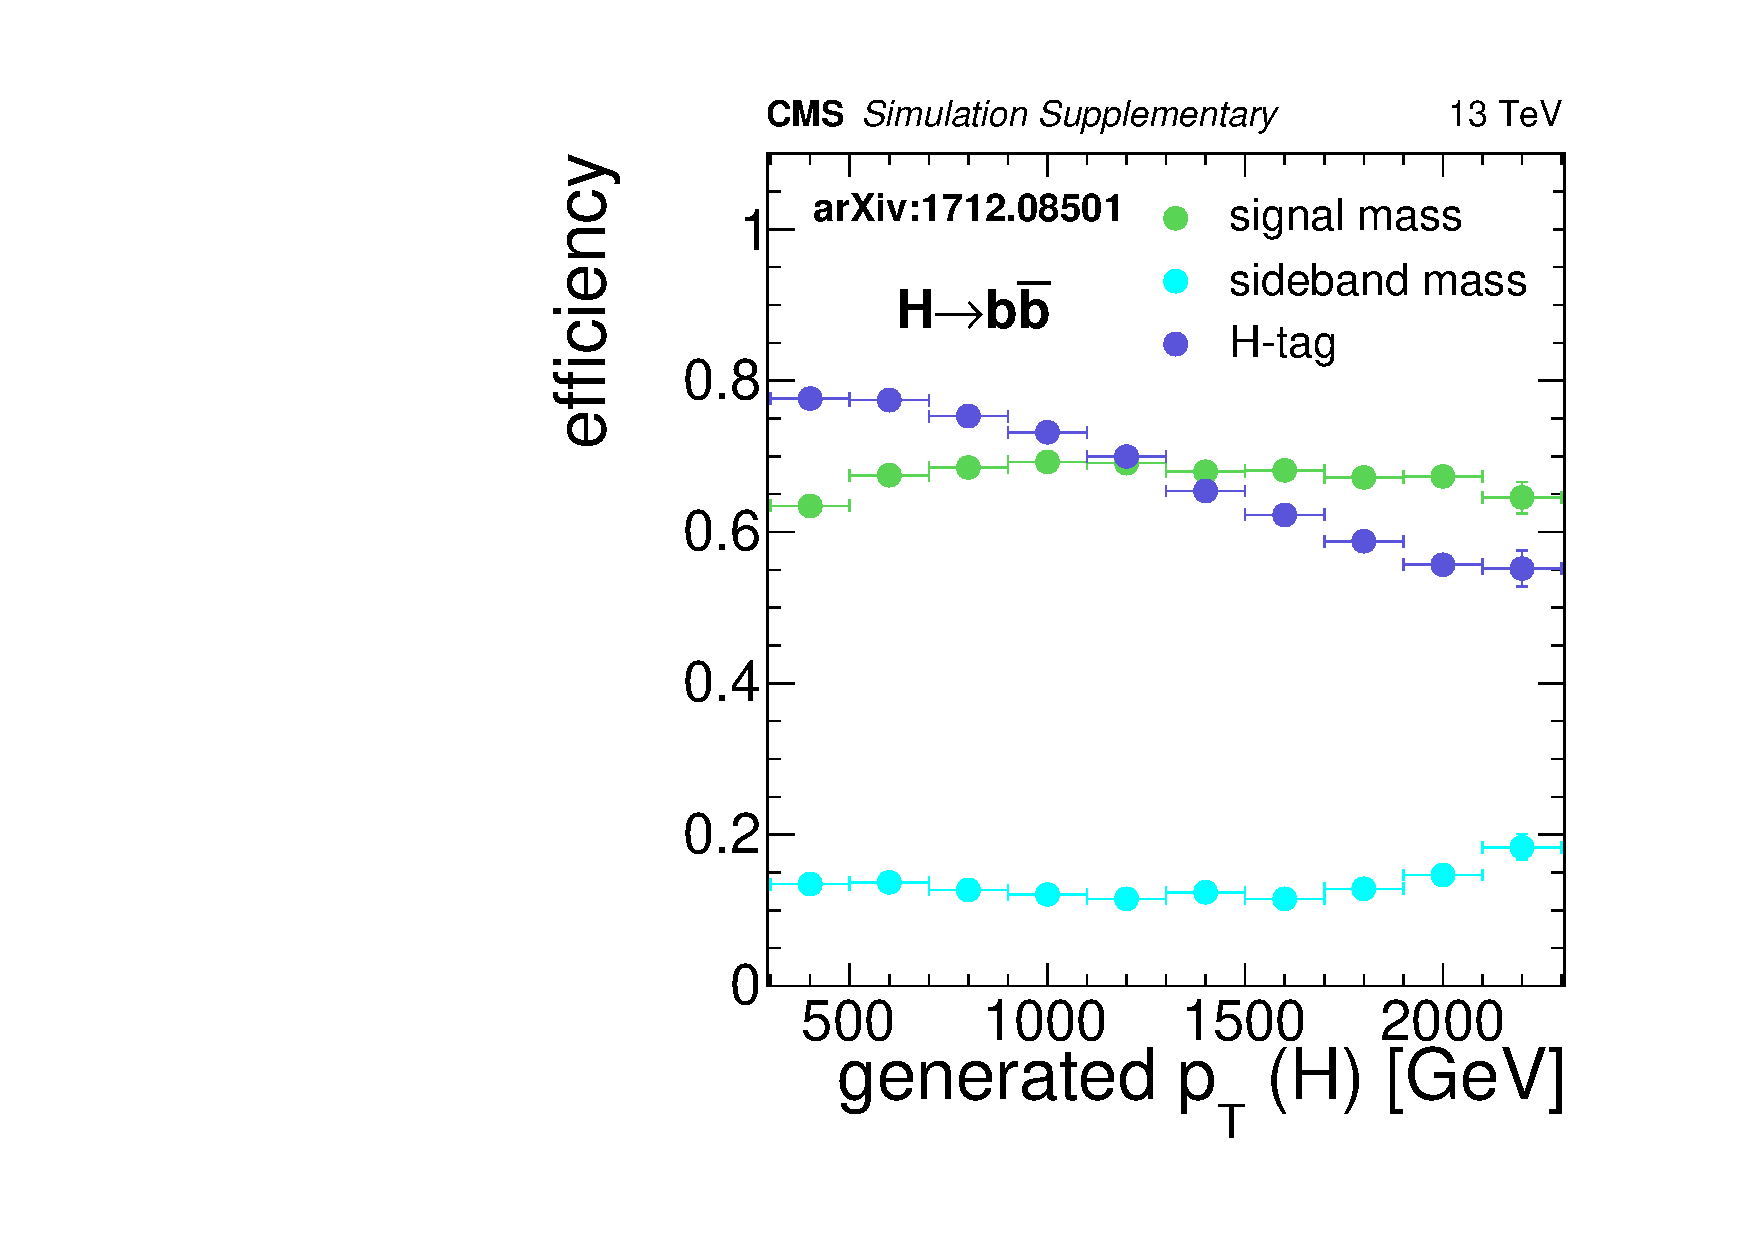
\includegraphics[width=0.45\linewidth]{figs/SUS17006/CMS-SUS-17-006_Figure-aux_006.pdf}
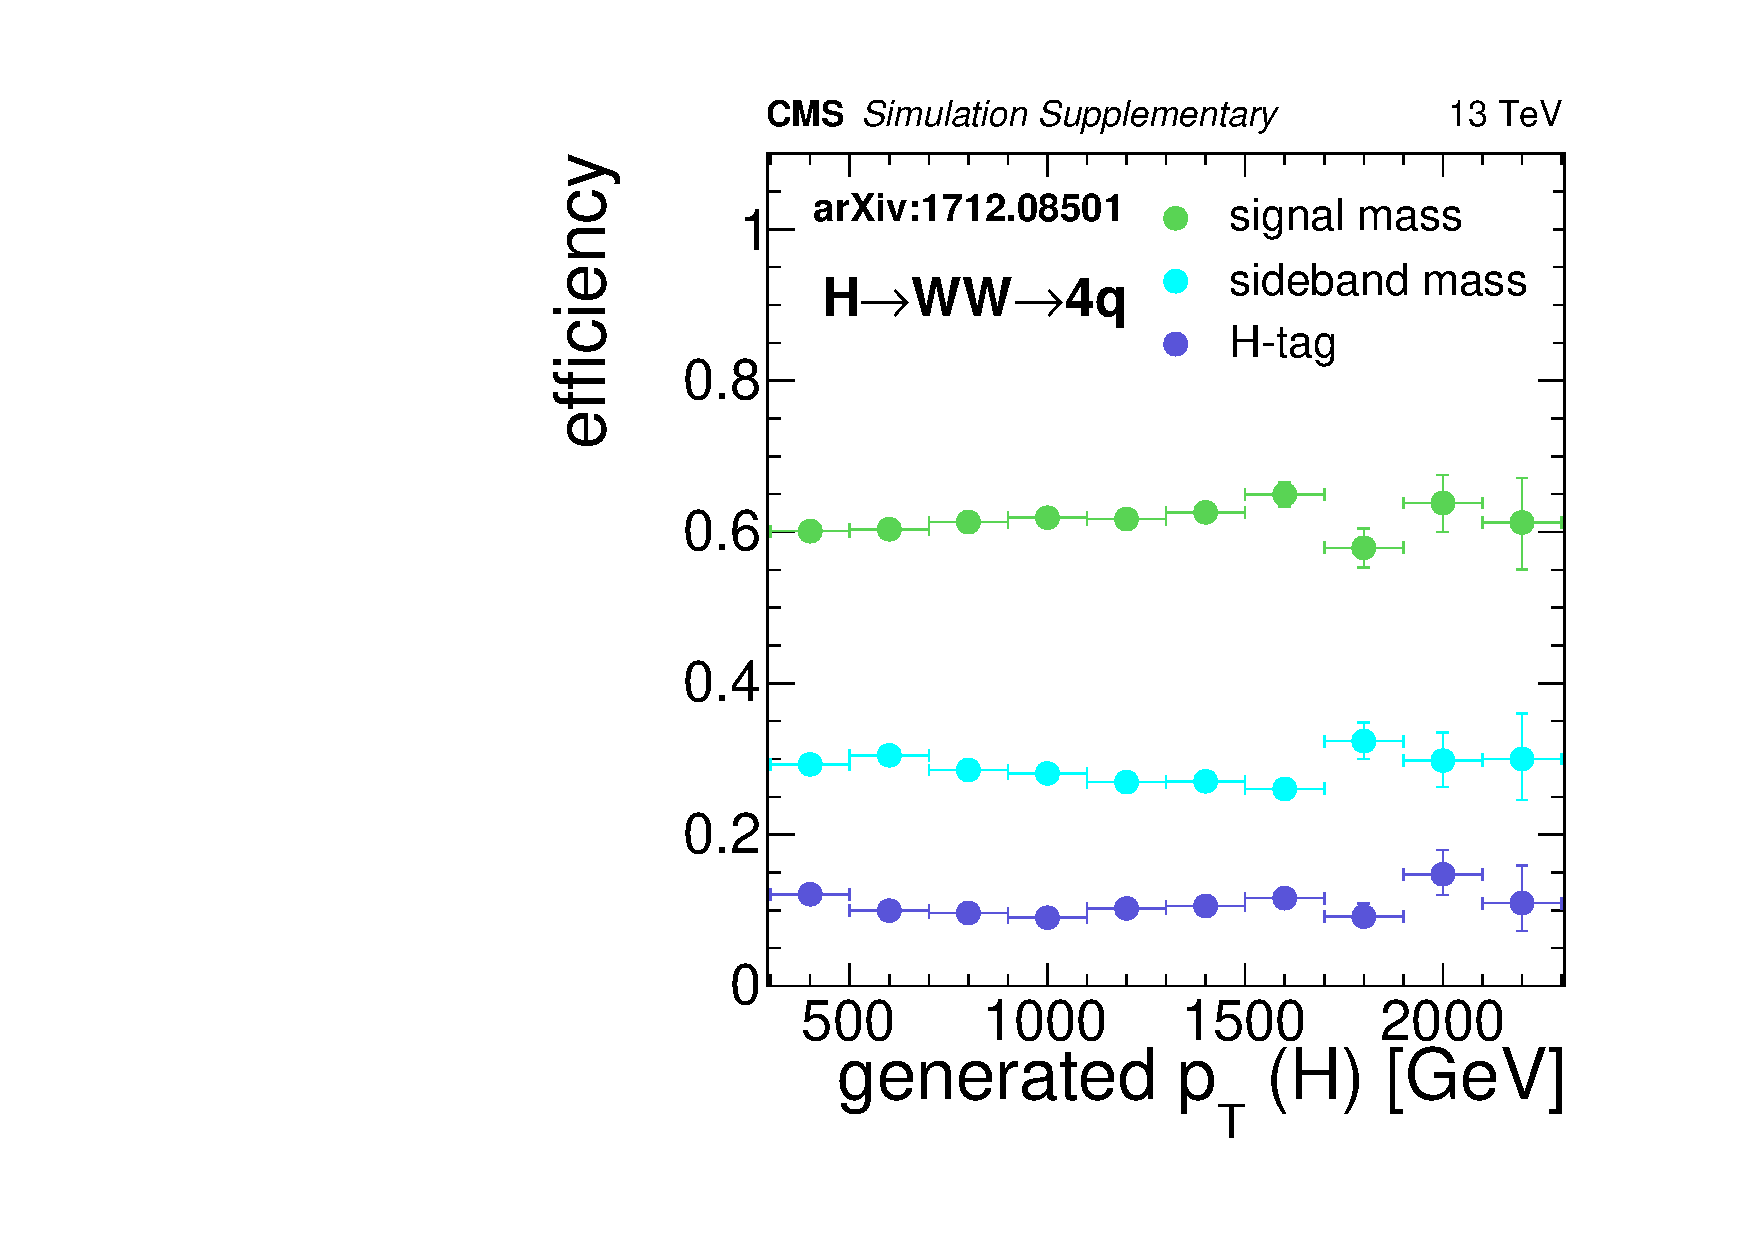
\includegraphics[width=0.45\linewidth]{figs/SUS17006/CMS-SUS-17-006_Figure-aux_007.pdf}\\
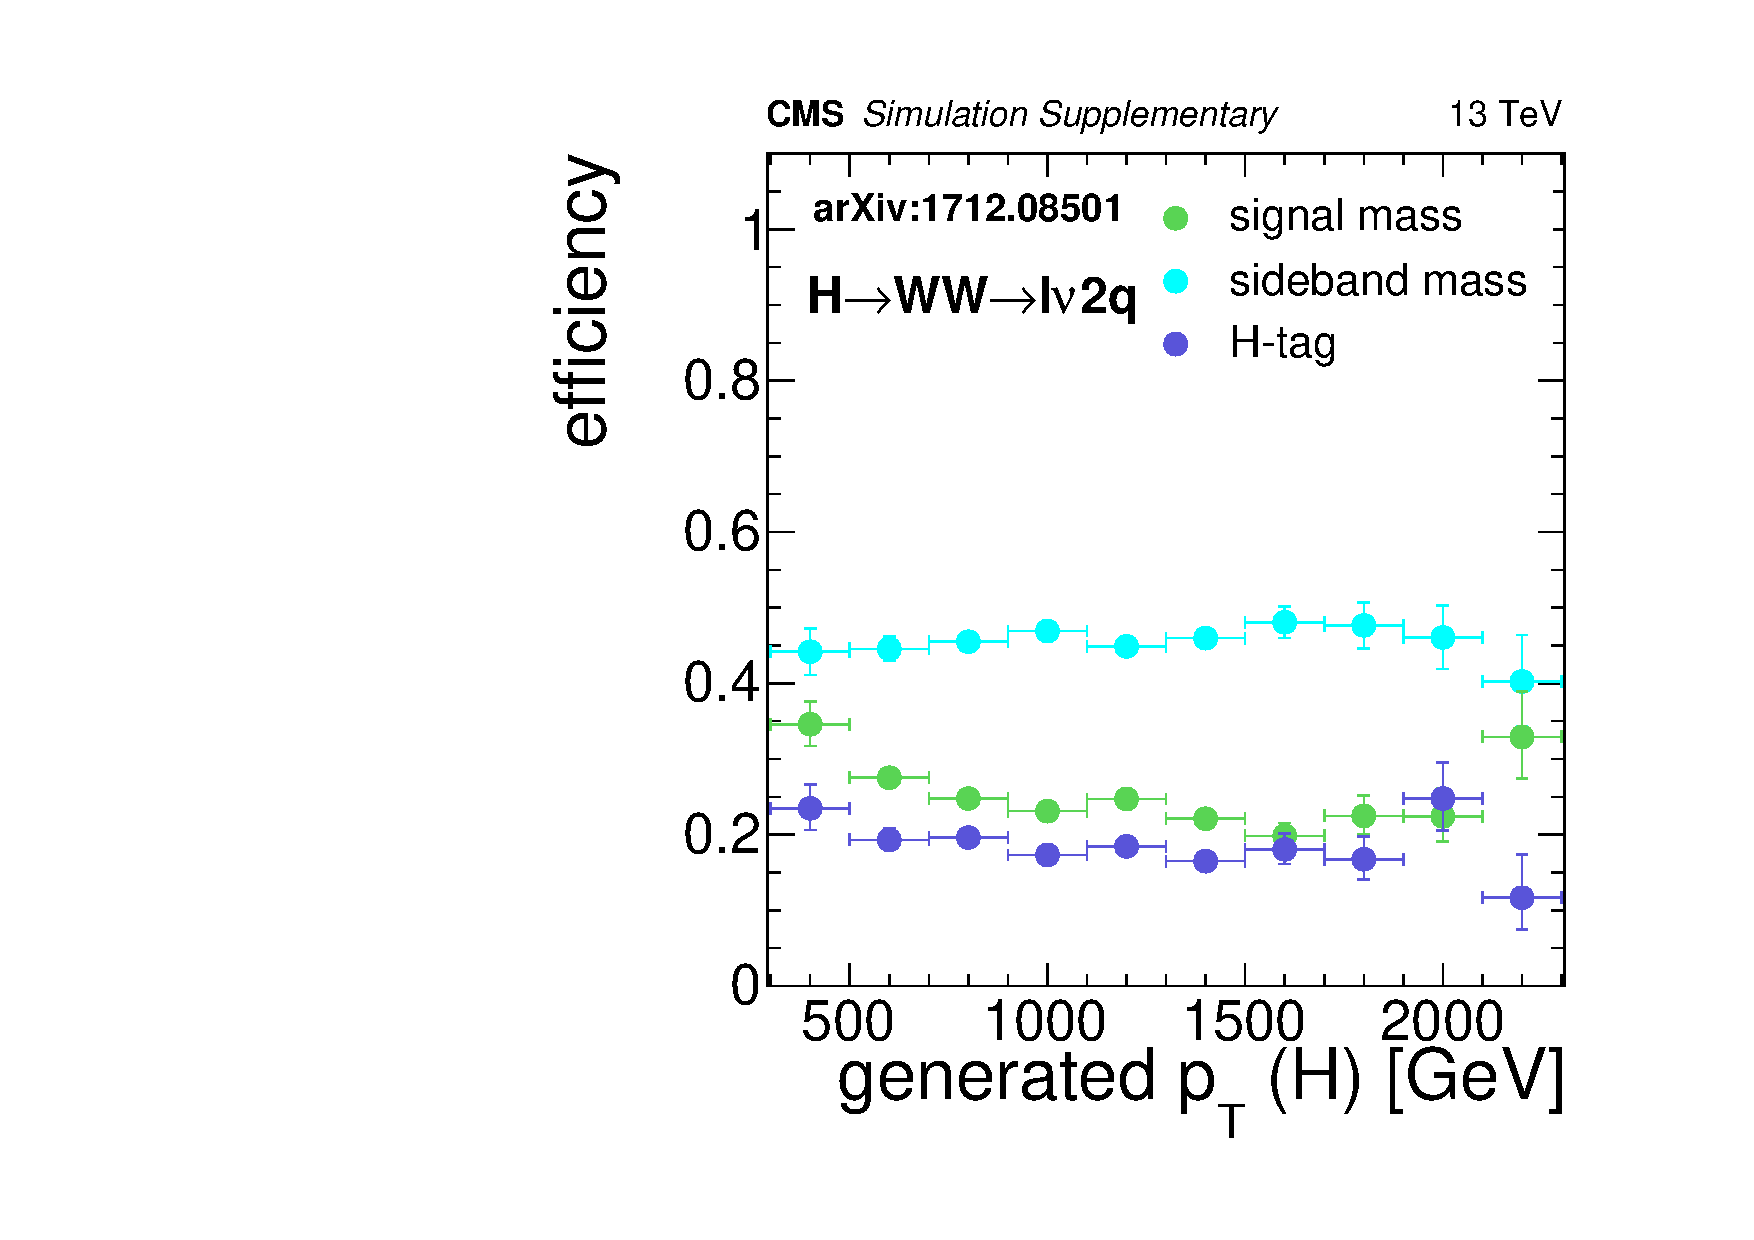
\includegraphics[width=0.45\linewidth]{figs/SUS17006/CMS-SUS-17-006_Figure-aux_008.pdf}
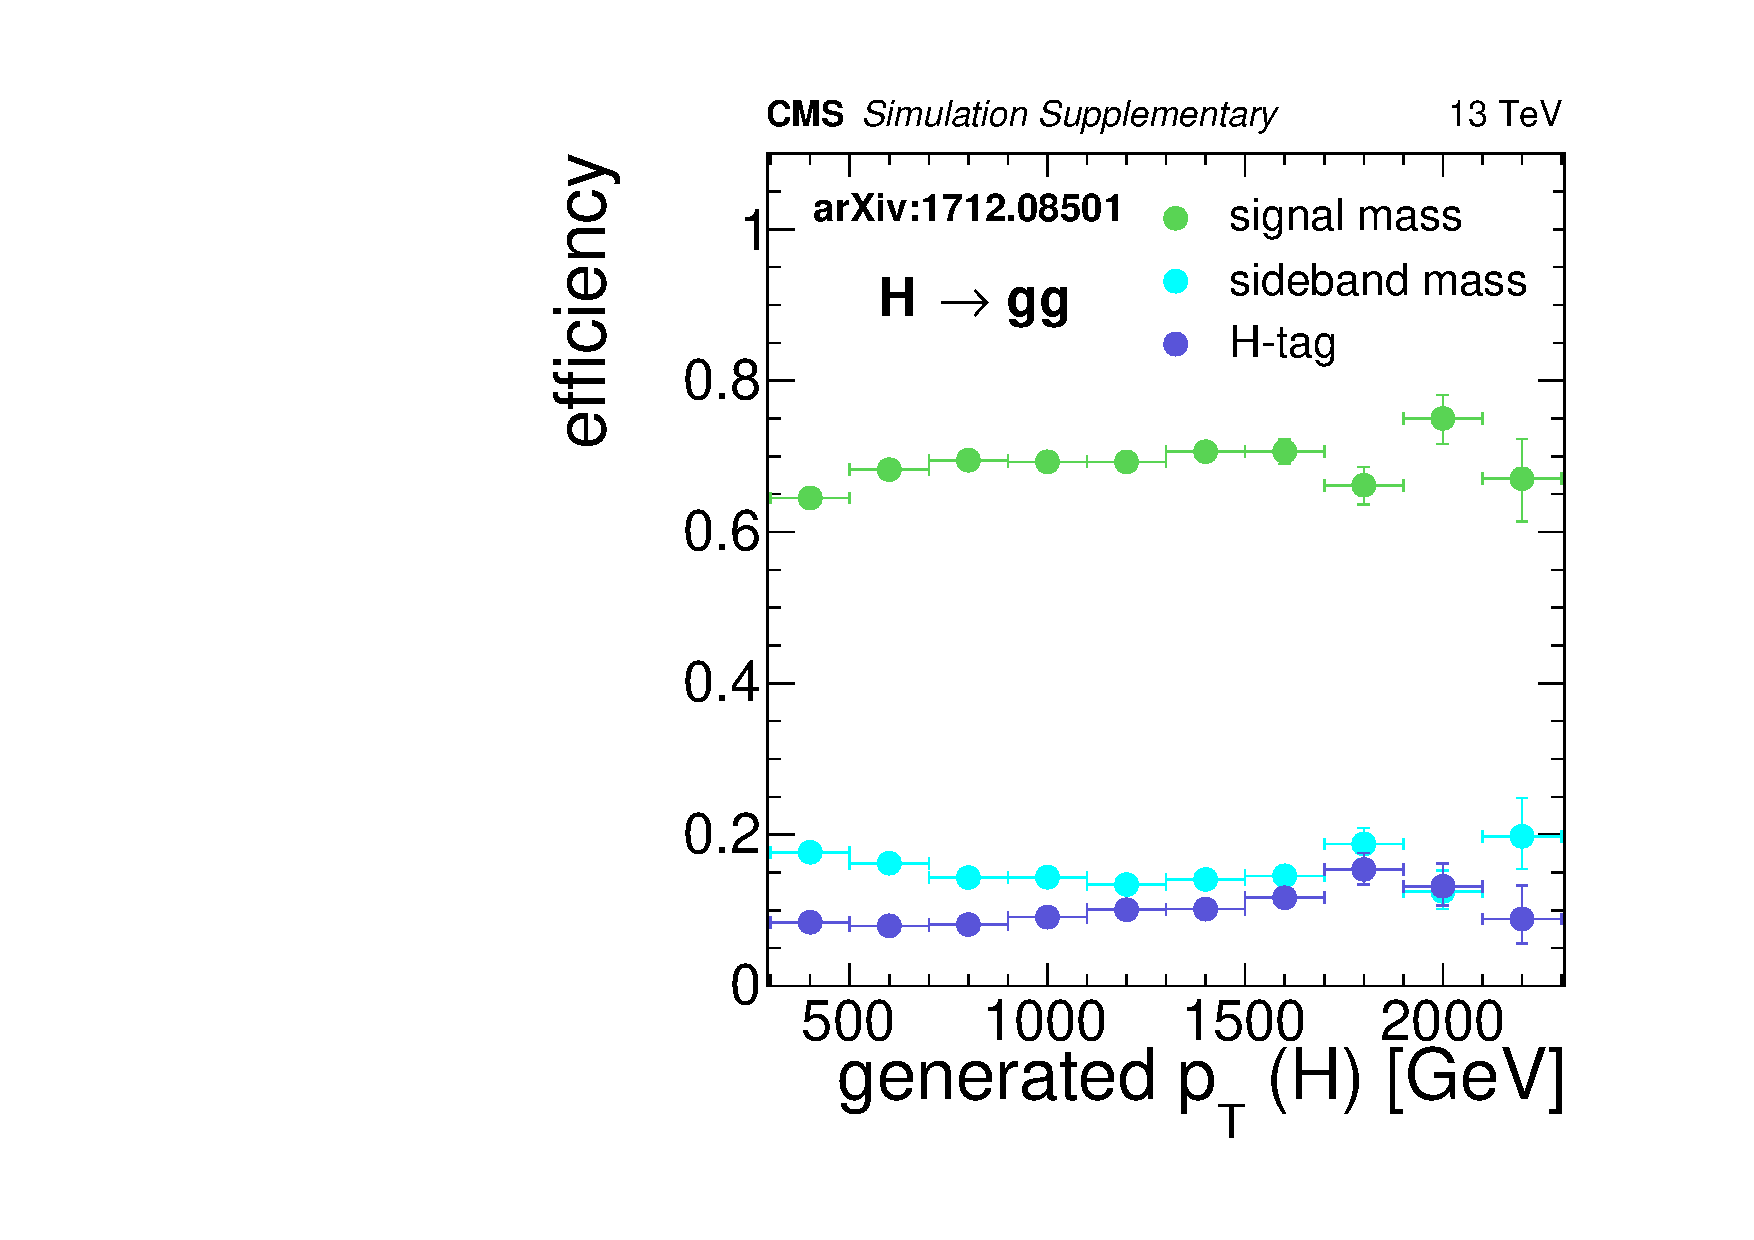
\includegraphics[width=0.45\linewidth]{figs/SUS17006/CMS-SUS-17-006_Figure-aux_009.pdf}
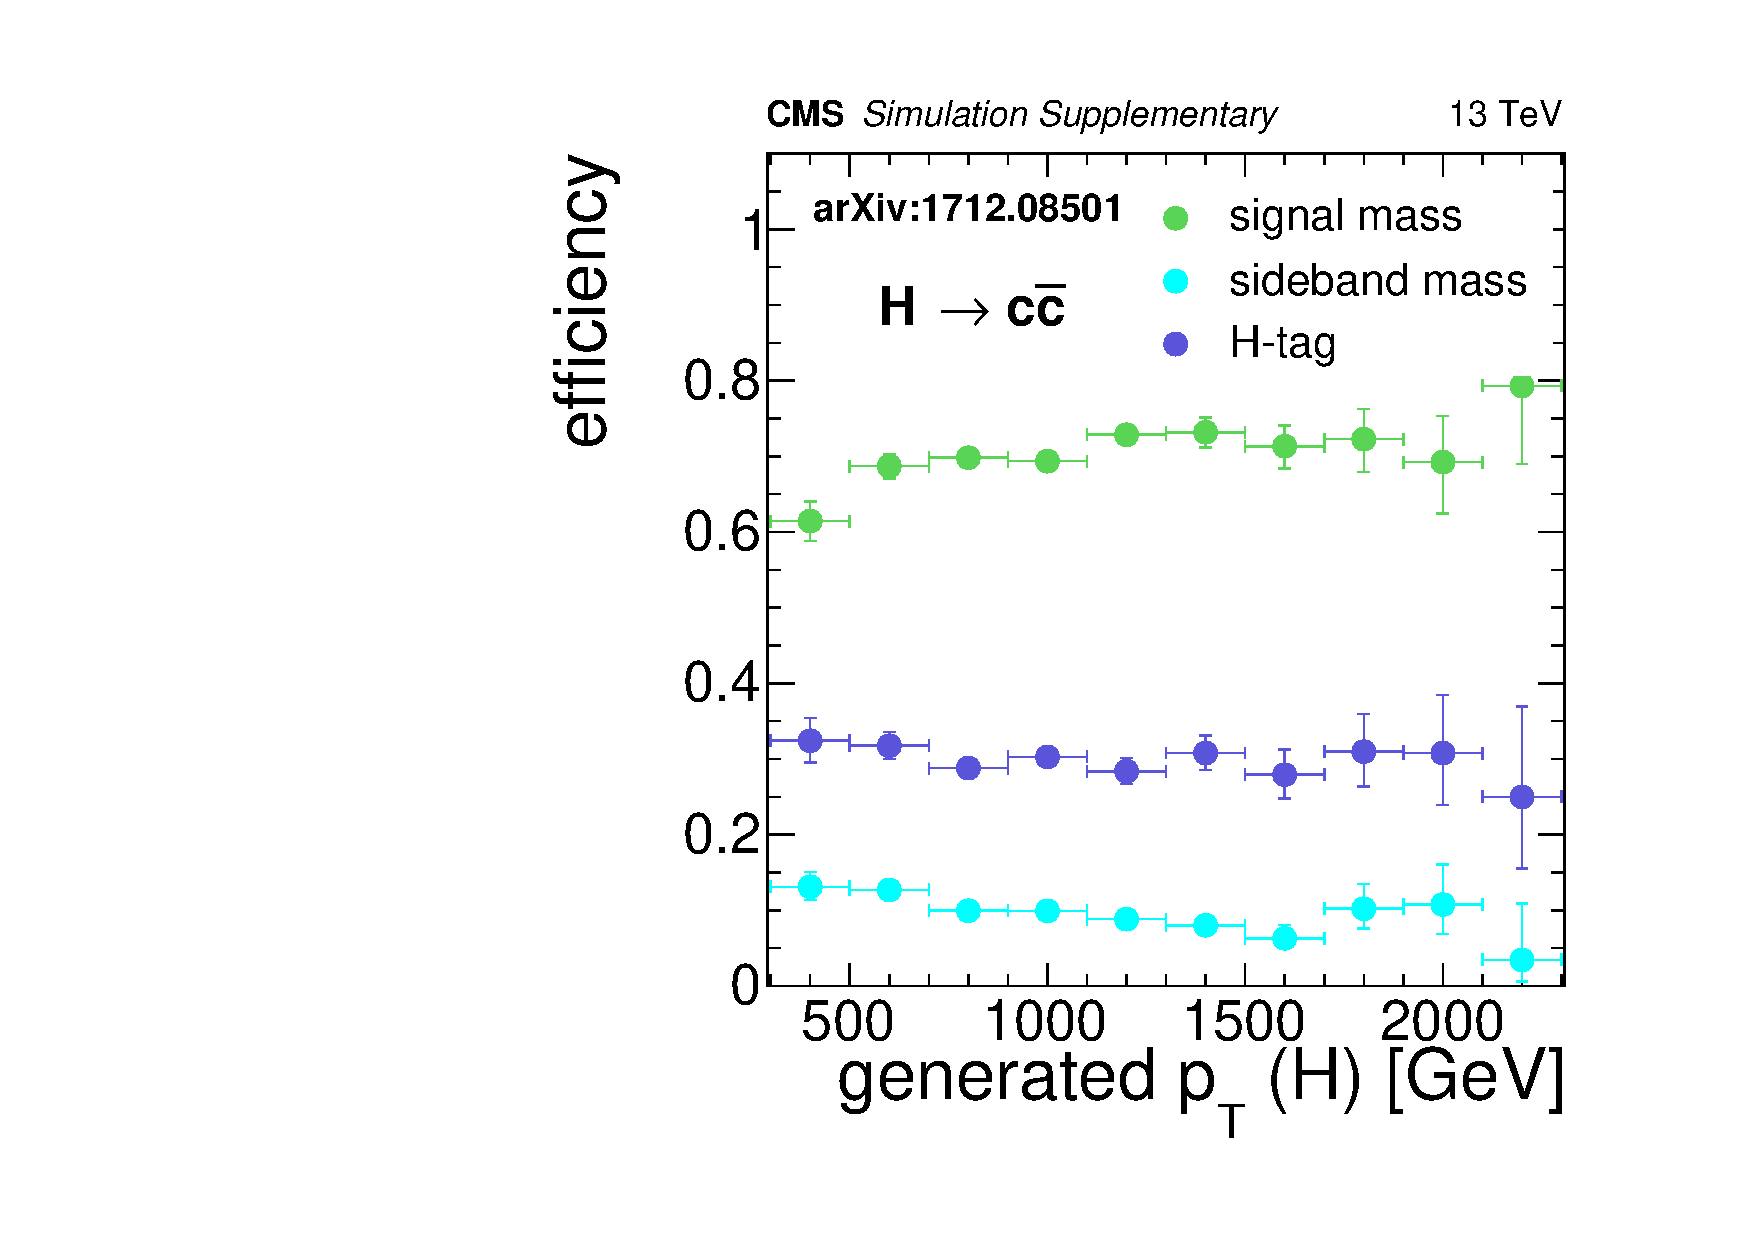
\includegraphics[width=0.45\linewidth]{figs/SUS17006/CMS-SUS-17-006_Figure-aux_010.pdf}
\caption{
Efficiencies for an AK8 jet originating from Higgs boson decay, relative to baseline selection.
The "signal mass" curve represents the probability the jet will fall within the mass region [85, 135 GeV].
The "sideband mass" curve represents the probability the jet will fall within the mass region [50, 85 GeV] or [135, 250 GeV].
The "H-tag" curve represents the probability the jet have a double-b discriminator value greater than 0.3, for jets within the mass region [50, 250 GeV].
The efficiencies were derived using the T5qqqqZH MC with a gluino mass of 2200 GeV.
}
\label{fig:effH}
\end{figure}

\begin{figure}
\centering
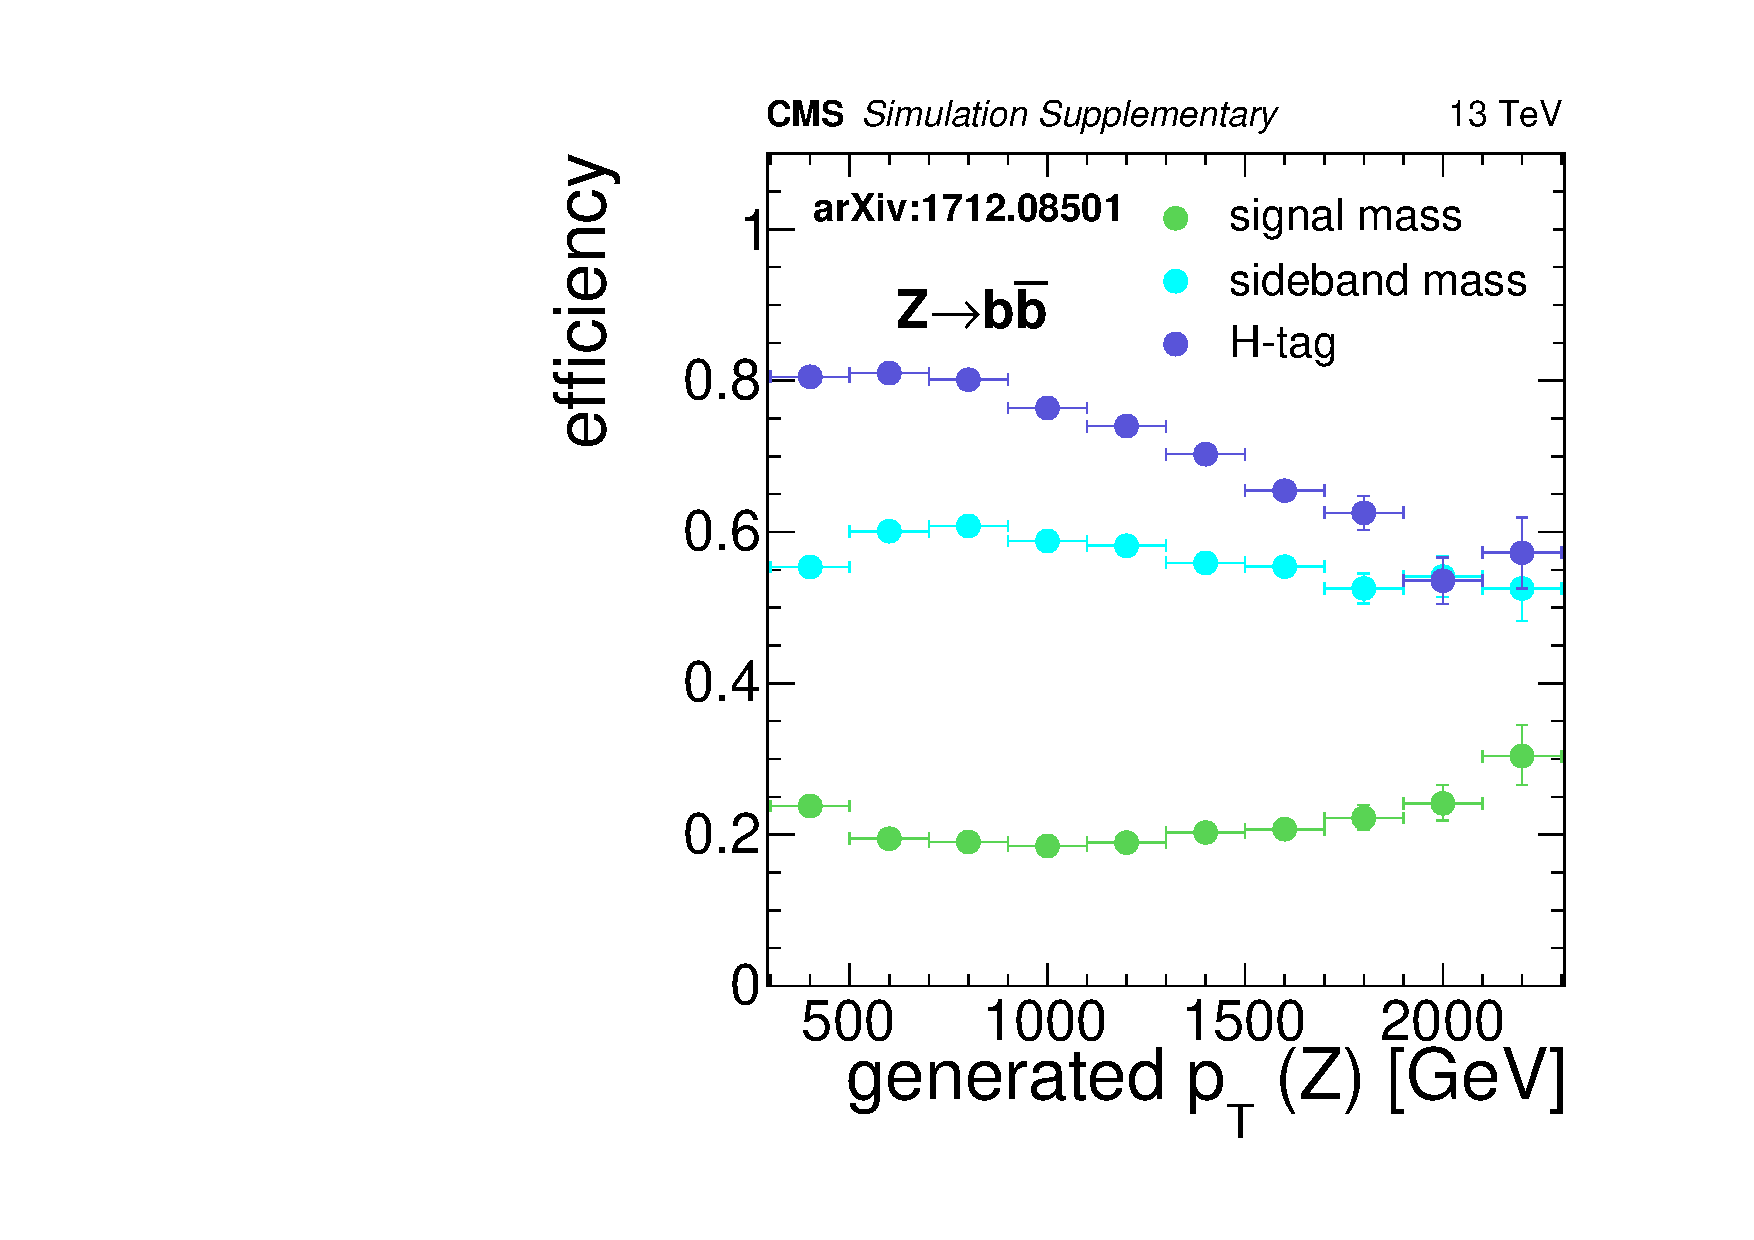
\includegraphics[width=0.45\linewidth]{figs/SUS17006/CMS-SUS-17-006_Figure-aux_011.pdf}
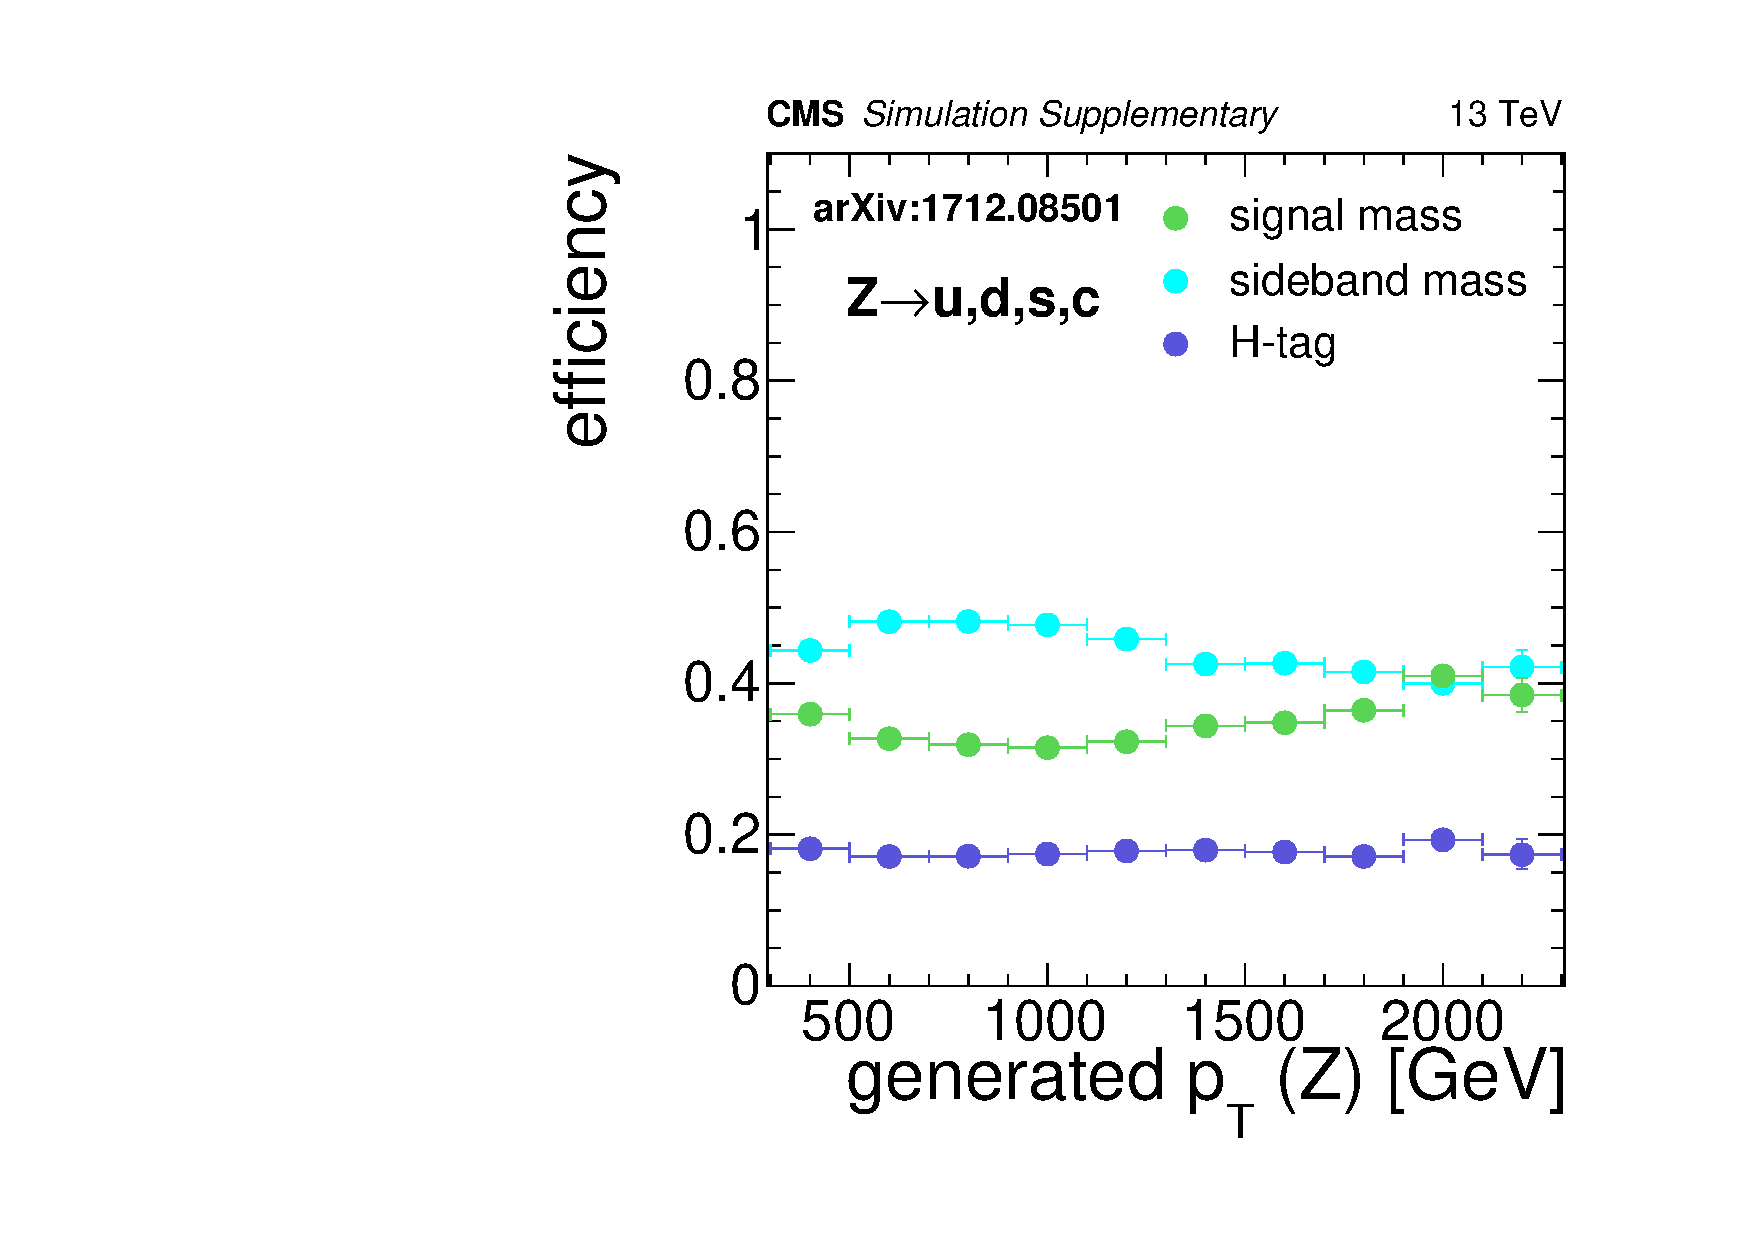
\includegraphics[width=0.45\linewidth]{figs/SUS17006/CMS-SUS-17-006_Figure-aux_012.pdf}\\
\caption{
Efficiencies for an AK8 jet originating from Z boson decay, relative to baseline selection.
The "signal mass" curve represents the probability the jet will fall within the mass region [85, 135 GeV].
The "sideband mass" curve represents the probability the jet will fall within the mass region [50, 85 GeV] or [135, 250 GeV].
The "H-tag" curve represents the probability the jet have a double-b discriminator value greater than 0.3, for jets within the mass region [50, 250 GeV].
The efficiencies were derived using the T5qqqqZH MC with a gluino mass of 2200 GeV.
}
\label{fig:effZ}
\end{figure}

\begin{table}
\centering
\caption{
Comparison of the true reco-level event yield with those obtained via the prediction following the prescription above.
The columns with the RECO or GEN labels are the prediction using RECO or GEN event variables only, respectively.
The prediction was made using the T5qqqqHH MC with a gluino mass of 2200 GeV.
}
%\begin{tabular}{c | c c c c c}
%\hline\hline
%            & RECO      & RECO                     & RECO          & GEN                        &  GEN\\
%            & "truth"   & \textbackslash w padding & no padding    & \textbackslash w padding   & no padding\\
%\hline
%Baseline    & 4.08      & 3.90 (-4.5\%)            & 3.46 (-15\%)  & 4.17 (+2.2\%)              &  3.53 (-16\%)\\
%A1          & 1.21      & 1.26 (+3.7\%)            & 1.18 (-2.3\%) & 1.36 (+11\%)               & 1.26 (+3.6\%)\\
%A2          & .777      & .821 (+5.7\%)            & .748 (-3.7\%) & .922 (+16\%)               & .815 (+4.7\%)\\
%B1          & .802      & .776 (-3.3\%)            & .703 (-12\%)  & .771 (-4.1\%)              & .664 (-21\%)\\
%B2          & .322      & .411 (+28\%)             & .338 (+5.0\%) & .457 (+30\%)               & .350 (+8.2\%)\\
%C           & .498      & .546 (+9.7\%)            & .473 (-4.9\%) & .594 (+16\%)               & .487 (-2.1\%)\\
%D           & .478      & .426 (-9.5\%)            & .353 (25\%)   & .415 (-15\%)               & .308 (-36\%)\\
\begin{tabular}{c | c c c}
\hline\hline
         & RECO     & RECO           & GEN\\
         & "truth"  & prediction     & prediction\\
\hline
Baseline & 4.08     & 3.46 (-15\%)   & 3.53 (-16\%)\\
A1       & 1.21     & 1.18 (-2.3\%)  & 1.26 (+3.6\%)\\
A2       & 0.777    & 0.748 (-3.7\%) & 0.815 (+4.7\%)\\
B1       & 0.802    & 0.703 (-12\%)  & 0.664 (-21\%)\\
B2       & 0.322    & 0.338 (+5.0\%) & 0.350 (+8.2\%)\\
C        & 0.498    & 0.473 (-4.9\%) & 0.487 (-2.1\%)\\
D        & 0.478    & 0.353 (25\%)   & 0.308 (-36\%)\\
\hline\hline
\end{tabular}
\label{tab:predclos}
\end{table}

\begin{table}
\centering
\caption{
Signal efficiencies for an event to land in a given analysis bin.
The efficiencies were derived using the T5qqqqHH MC with a gluino mass of 2200 GeV.
Choosing a gluino mass of 1800 GeV decreases the efficiencies by a relative 5\%.
}
\begin{tabular}{c | c c c c c c c c}
\hline
\hline
                                                            & Baseline & A1     & A2      & B1      & B2      & C       & D\\
\hline
$p_{\mathrm{T}}^{\mathrm{miss}} < 300\,\mathrm{GeV}$        & 32\%    & 9.4\%   & 6.0\%   & 6.2\%   & 2.5\%   & 3.9\%   & 3.7\% \\
$300 < p_{\mathrm{T}}^{\mathrm{miss}} < 500\,\mathrm{GeV}$  & 2.7\%   & 0.78\%  & 0.52\%  & 0.54\%  & 0.25\%  & 0.31\%  & 0.30\% \\
$500 < p_{\mathrm{T}}^{\mathrm{miss}} < 700\,\mathrm{GeV}$  & 3.5\%   & 1.0\%   & 0.65\%  & 0.72\%  & 0.28\%  & 0.43\%  & 0.40\% \\
$p_{\mathrm{T}}^{\mathrm{miss}} > 700\,\mathrm{GeV}$        & 26\%    & 7.6\%   & 4.9\%   & 5.0\%   & 2.0\%   & 3.1\%   & 3.0\% \\
\hline
\hline
\end{tabular}
\label{tab:sigeff}
\end{table}

\section{Conclusions}
